\documentclass{classes/SIT-Report-EN}
\usepackage{tabularx}
\usepackage{graphicx}
\usepackage{adjustbox}
\usepackage{lscape}
\usepackage{longtable}
\usepackage{tabularray}
\usepackage{color}
\usepackage{multirow}
\usepackage{graphicx}
\usepackage[normalem]{ulem}
\usepackage{hyperref}
\usepackage{filecontents}
\usepackage{needspace}
\usepackage{array}
\useunder{\uline}{\ul}{}
 
%%Edit your info Here
\begin{document}
\title{LOSTNFOUND KMUTT: KEEP A CLOSE EYE ON YOUR ITEMS.}
\titleTH{ลอสท์แอนด์ฟาวด์ มจธ.}
\degree{Bachelor of Science}
\majorProgramEN{Computer Science}
\academicyear{2024}

\author{MR.PASSAKORN PUTTAMA}
\authorTwo{MR.VATCHARAMAI RODRING}
\authorThree{MR.PATTHADOL RAKSAPRAM}

\majoradvisor{Asst.Prof. Worarat Krathu Ph.D}
\committeeOne{Dr. Watanyoo Suksa-ngaim Ph.D}
\committeeTwo{Dr. Vithida Chongsuphajaisiddhi Ph.D}
\academicyear{2024}

%%%%%%%%%%
\maketitle
\frontmatter
\maketitleinner
\makeapproval
% ************************** Thesis Abstract **********************************
\begin{abstract}
\par
LostNFound KMUTT is a web-based platform designed to assist KMUTT students and university personnel in efficiently managing lost and found items within the university. The platform allows users to report lost or found items through dedicated forms, providing item descriptions, locations, and timestamps for precise matching. It utilizes advanced technologies such as Natural Language Processing (NLP) for text similarity matching and secure authentication via university email to ensure rightful ownership. Additionally, it features a history of claimed items for accountability and a notification system to remind users to retrieve their belongings promptly.

The development process demonstrates the feasibility of creating an efficient lost-and-found management system using existing university resources and modern web technologies. By streamlining the process, the platform minimizes user frustration and enhances operational productivity for KMUTT staff.
\vfill
\paragraph*{Keywords :} Lost and Found, KMUTT, Web Platform, Item Matching, Secure Claims
\vfill
\end{abstract} %%Edit your Abstract
% ************************** Thesis Acknowledgements **************************
\begin{acknowledgements}
\par
We received assistance and guidance from several respected persons, who deserve our deepest gratitude. This project would not have been possible without the support of Asst. Prof. Dr. Worarat Krathu and Dr. Watanyoo Suksa-ngaim contributed invaluable insight and experience.
\end{acknowledgements} %% %%Edit your Acknowledgement

\tableofcontents
\listoftables
\listoffigures
%% ***************************** Thesis Symbols ********************************
\begin{symbols}
    \noindent
    \begin{tabular*}{\textwidth}{@{}p{0.18\textwidth}p{0.8\textwidth}@{}}
        {$\theta$} & {Theta} \\
        {$d$} & {distance} \\
        {kg} & {Kilogram} \\
        {m$^{2}$} & {Square Metre} \\
    \end{tabular*}
\end{symbols}
%% ************************** Thesis Abbreviations **************************
\begin{abbreviations}
    \noindent
    \begin{tabular*}{\textwidth}{@{}p{0.18\textwidth}p{0.8\textwidth}@{}}
        {DoF} & {Degree of Freedom} \\
        {CoM} & {Center of Mass} \\
        {KMUTT} & {King Mongkut's University of Technology Thonburi} \\
    \end{tabular*}
\end{abbreviations}


\mainmatter
%%insert your content
\chapter{Introduction}

\section{Background}
Losing personal belongings within a university environment is a common challenge, and KMUTT is no exception. Currently, the recovery process involves contacting security personnel in different areas, which can be inefficient and inconvenient for both students and staff. This lack of a centralized system often leads to prolonged delays in retrieving lost items and potential frustrations for the involved parties.

To address these issues, the LostNFound KMUTT platform aims to streamline and enhance the lost-and-found process through a centralized web-based solution. By utilizing modern web technologies and intelligent text-matching models, this platform simplifies reporting, cataloging, and locating lost items.

\section{Objective}
To create a user-friendly and efficient platform that facilitates the reporting and retrieval of lost items. By integrating modern technology into the existing process, we aim to reduce the complexities associated with lost and found items, making it easier for both users and officers to manage and locate belongings promptly.

\section{Expected Benefits}
\begin{enumerate}
    \item \textbf{Efficiency Improvement:} Reduced processing time for reporting, cataloging, and retrieving lost items.
    \item \textbf{User Convenience:} Accessible information through a user-friendly interface.
    \item \textbf{Enhanced Security:} Robust identity verification to ensure rightful ownership.
    \item \textbf{Reduced Frustration:} Simplified processes for users and staff.
    \item \textbf{Resource Optimization:} Improved productivity for staff by automating processes.
    \item \textbf{Timely Notifications:} Notifications to remind users to pick up their items.
    \item \textbf{Documentation and Accountability:} Comprehensive records of claimed items for auditing.
\end{enumerate}

\section{Scope}
\subsection{Target}
King Mongkut's University of Technology Thonburi (KMUTT).

\subsection{Scope of Work}
\begin{enumerate}
    \item Define Project Features:
    \begin{itemize}
        \item \textbf{Distinct Features:}
        \begin{enumerate}
            \item Item Found \& Lost Form: Allow users who found or lost items to report them, providing the time and location where it was found and describing the item to enable matching.
                \begin{itemize}
                    \item Found Item Form.
                    \item Lost Item Form.
                \end{itemize}
            \item Claim Process: Allow users to claim found items after the form is matched.
                \begin{itemize}
                    \item Text comparison using Natural Language Processing (NLP).
                    \item Notification system.
                \end{itemize}
            \item Secure Items Ownership: Prevent unauthorized claims using university email authentication.
        \end{enumerate}
        \item \textbf{Support Features:}
        \begin{enumerate}
            \item Authentication using OAuth with Microsoft authentication.
            \item History of Claimed Items.
        \end{enumerate}
    \end{itemize}
    \item Architecture and Technology Stack:
    \begin{itemize}
        \item \textbf{Frontend:} Next.js 14.
        \item \textbf{Backend:} Next.js 14 and FastAPI.
        \item \textbf{Database:} PostgreSQL.
        \item \textbf{Authentication:} NextAuth.js with Microsoft as the provider.
        \item \textbf{Infrastructure:} Google Cloud (GCP), Docker.
        \item \textbf{Model:} Public text similarity and NER model from Hugging Face.
        \item \textbf{Testing:} Jest (Unit testing), Postman (API testing).
    \end{itemize}
\end{enumerate}



\chapter{Feasibility Study}

\section{Introduction}
The LostNFound platform is a centralized web application designed to address the challenges associated with managing lost-and-found items at King Mongkut's University of Technology Thonburi (KMUTT). The platform aims to provide students, staff, and university personnel with an efficient, accessible, and secure solution for reporting and reclaiming lost items.

Unlike the current manual and on-site processes, the LostNFound platform digitizes the entire lost-and-found workflow. Users can report lost items, search for them, and claim ownership through the platform, reducing time and effort. It also introduces features such as real-time item status updates, secure ownership verification, and centralized database management. This initiative aligns with KMUTT’s commitment to modernizing student services and fostering a more convenient university experience.

\section{Problem Statement}
Currently, KMUTT’s lost-and-found system relies on physical reporting to either nearby security personnel or the Student Affairs Division. This approach is inefficient, time-consuming, and prone to security risks such as unauthorized claims. The lack of a unified system makes tracking and managing lost items cumbersome for both users and staff. Furthermore, the absence of a centralized database means there is no effective way to ensure transparency or accessibility for all stakeholders.

The LostNFound platform aims to resolve these issues by providing a digital solution. The platform will centralize all lost-and-found operations, improve communication between stakeholders, and reduce the time required to locate and reclaim lost items. By introducing advanced features such as user profiles, secure claims verification, and automated notifications, the system will create a seamless experience for KMUTT’s community.

\section{Related Research and Projects}
\subsection{Lifeguard Lost \& Found}
A system designed to handle lost and found items in public spaces like airports and transport hubs, which shares similarities with the university setting. It allows users to report, search for, and claim items, ensuring secure ownership verification.

\subsection{MissingX}
A centralized platform for lost and found items, focusing on automatic matching of lost and found property. The platform also supports user notifications when a match is made, aligning with this system’s goal of real-time updates and seamless matching.

\subsection{ItemFinder}
Designed specifically for institutions like universities, ItemFinder handles lost and found items by providing a centralized platform for reporting, cataloging, and verifying items.

\subsection{Comparison of Existing Functions}
\begin{table}[h!]
\centering
\caption{Existing Functions of Related Applications}
\begin{tabular}{|l|c|c|c|c|c|}
\hline
\textbf{Applications} & \textbf{Item Reporting} & \textbf{Matching (NLP)} & \textbf{Notifications} & \textbf{History of Claims} & \textbf{User Profiles} \\
\hline
Lifeguard Lost \& Found & Yes & No & No & No & No \\
\hline
MissingX & Yes & Yes & Yes & No & No \\
\hline
ItemFinder & Yes & No & No & No & Yes \\
\hline
LostNFound KMUTT & Yes & Yes & Yes & Yes & Yes \\
\hline
\end{tabular}
\end{table}

\section{Requirement Specifications}
\subsection{Functional Requirements}
\begin{enumerate}
    \item Report lost and found items by filling out a form with details such as item description, location, and time.
    \item Provide real-time updates regarding the status of items.
    \item Use Natural Language Processing (NLP) to match descriptions of lost and found items.
    \item Notify users when a match is found for their lost item or when their claimed item is ready for pickup.
    \item Maintain a history of claimed items, including photos and verification details.
    \item Integrate with the university’s email system (OAuth with Microsoft) for authentication and ownership verification.
\end{enumerate}

\subsection{Data Requirements}
\begin{enumerate}
    \item \textbf{User Information:} Collect and store user details (e.g., phone number, university email, profile information, claim history) for authentication and personalized user experience.
    \item \textbf{Item Information:} Store details of each lost and found item, including item type, description, location, date, and images.
\end{enumerate}

\section{Implementation Techniques}
\subsection{Frontend}
\begin{itemize}
    \item Programming Language: TypeScript.
    \item Framework: Next.js.
\end{itemize}

\subsection{Backend}
\begin{itemize}
    \item Programming Language: TypeScript, Python.
    \item Frameworks: Next.js, FastAPI.
\end{itemize}

\subsection{Infrastructure}
\begin{itemize}
    \item OS: Debian Linux.
    \item Cloud Provider: Google Cloud Platform (GCP).
    \item Containerization: Docker.
    \item CI/CD: Google Cloud Build.
    \item Deployment Platform: Google Cloud Run.
\end{itemize}

\subsection{Database}
\begin{itemize}
    \item Database Type: Relational (PostgreSQL).
\end{itemize}

\subsection{Testing}
\begin{itemize}
    \item Unit Testing: Jest.
    \item API Testing: Postman.
\end{itemize}

\chapter{Analysis and Design}
\section{Introduction}
\par
This chapters covers three topics which are user requirement, business process designs, and system design. The user requirement part discusses the business needs for what users require from the system, The business process design part discusses the activities diagram, use case diagram, and context diagram of the application. Lastly, the system design consists of database design, and system architecture.

\section{User definition}
\begin{itemize}
    \item People who aged around 12 - 40 years old and familiar with English language
    \item Lived in Bangkok and in the city crowded with technology-accessible people
    \item People who trying to travel into newly visited place without known directions
    \item People who want to browse alternative transportation method to reach their destination with their own condition like cost savings, faster route, or less transfer
\end{itemize}
\subsection{User persona}
\begin{figure}[!h]
    \centering
    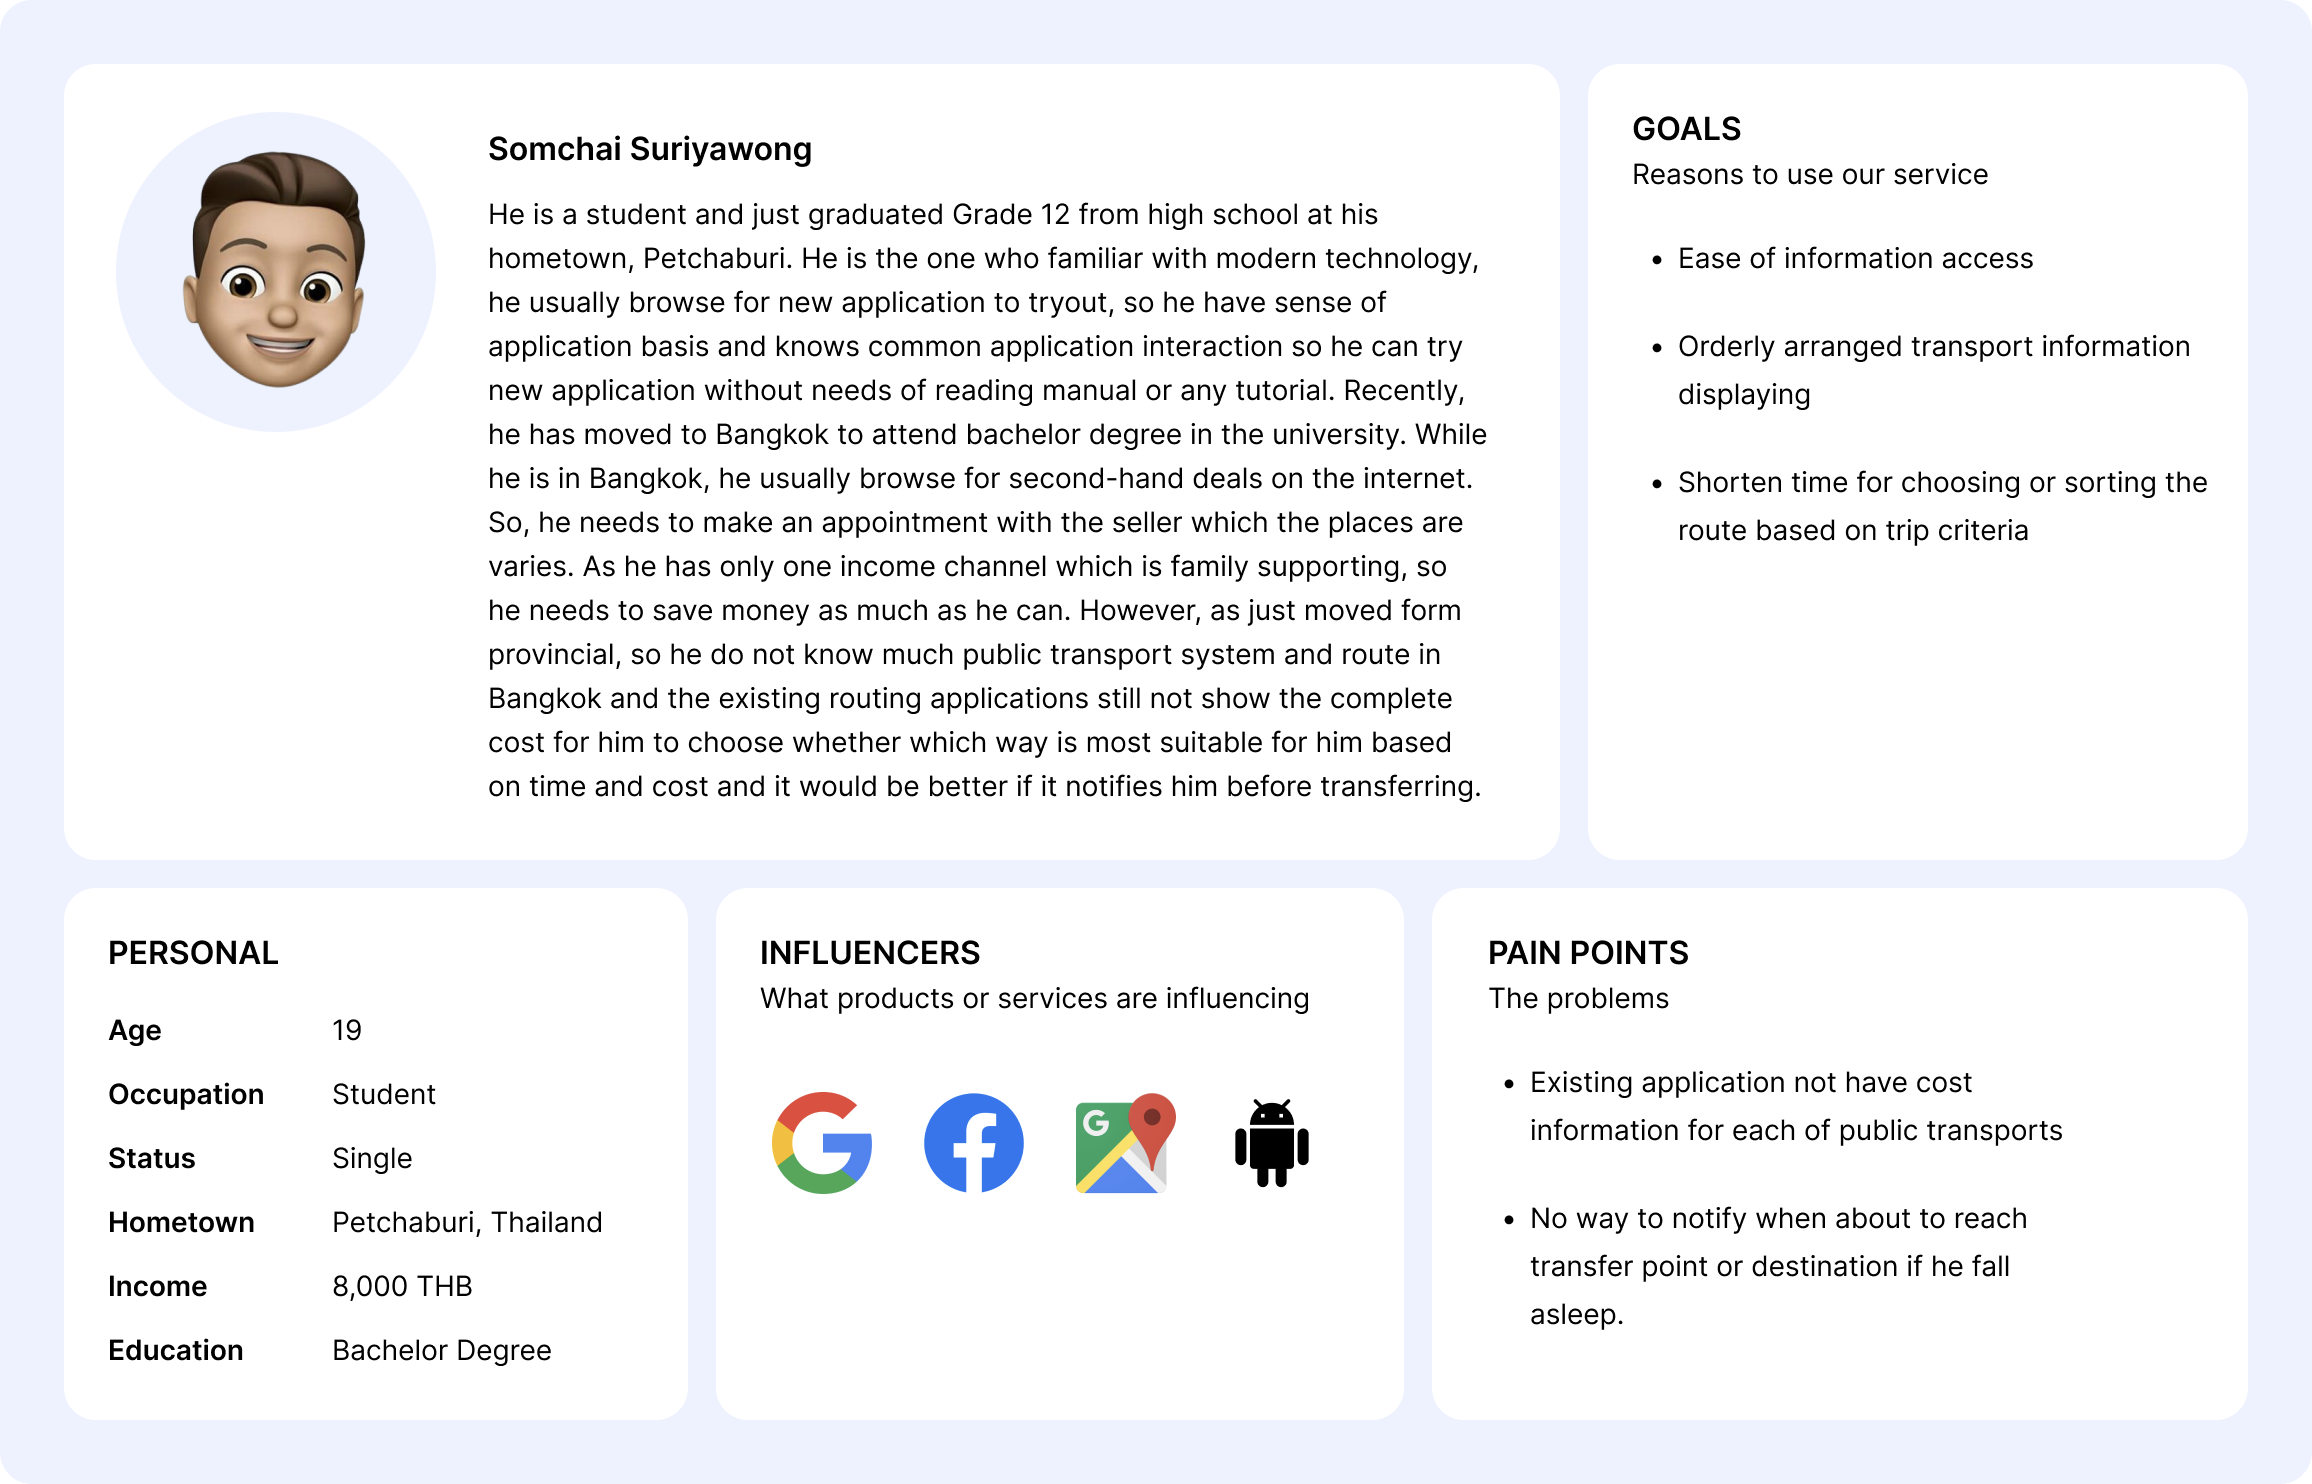
\includegraphics[width=1\linewidth]{chapter3/user-persona-1.png}
    \caption{User one persona}    
    \label{fig:User one persona}
\end{figure}
\begin{figure}[!h]
    \centering
    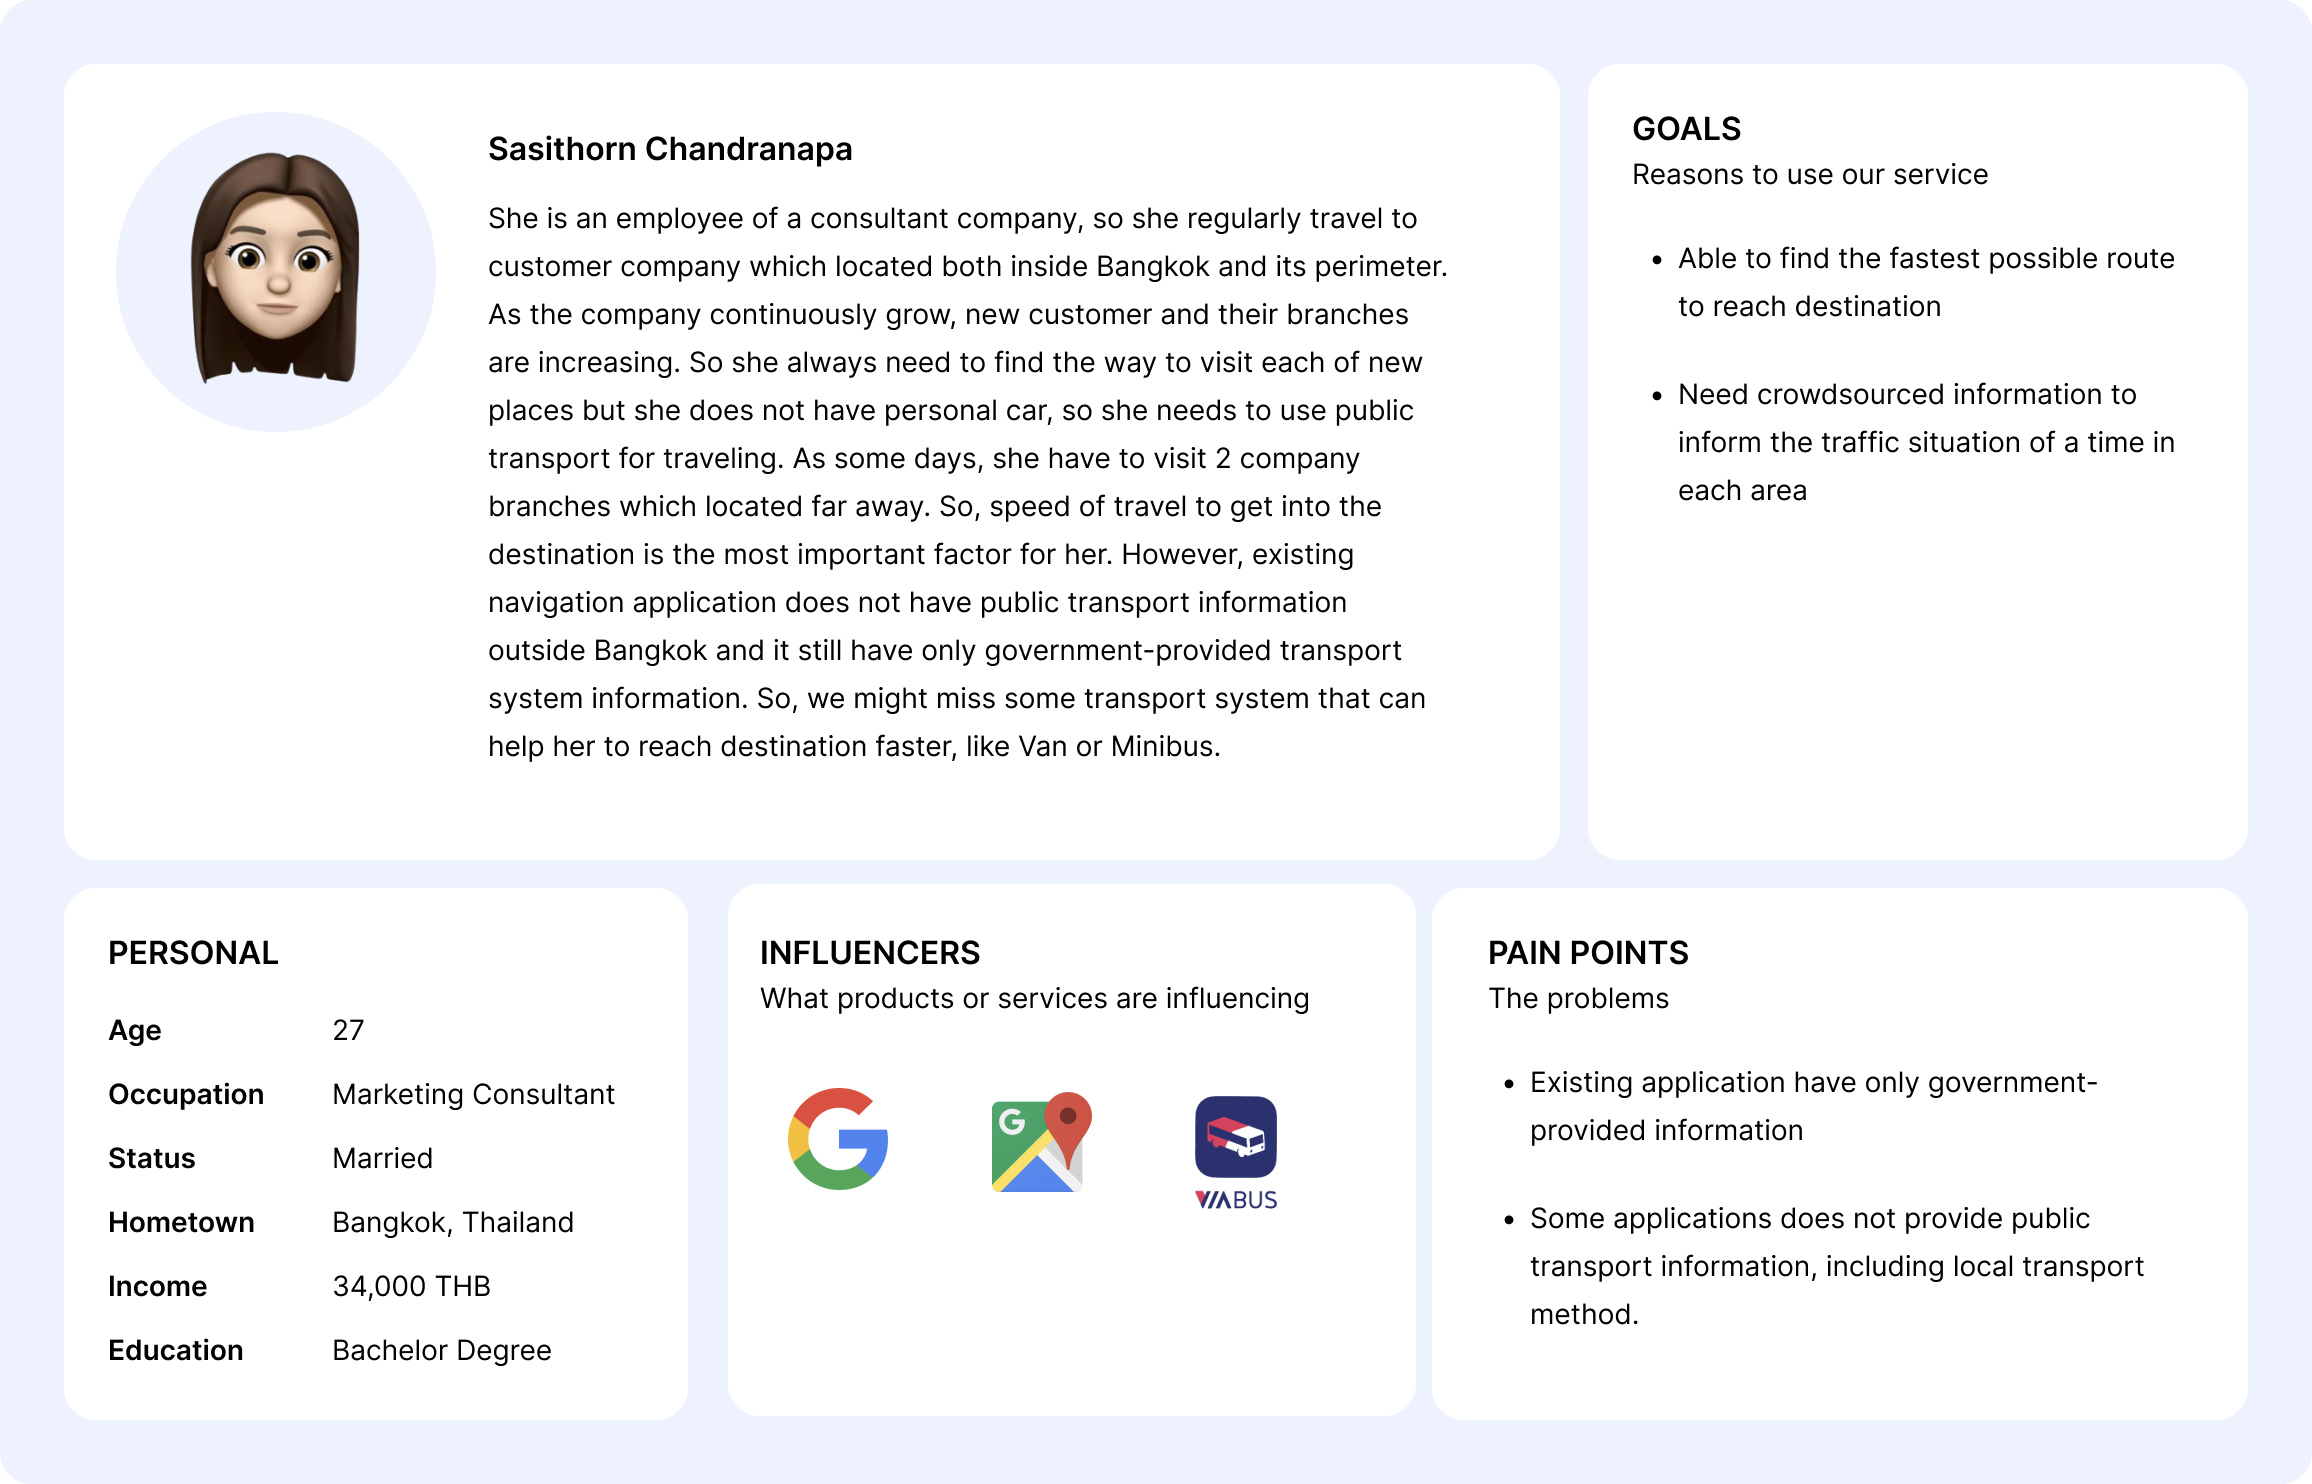
\includegraphics[width=1\linewidth]{chapter3/user-persona-2.png}
    \caption{User two persona}
    \label{fig:User two persona}
\end{figure}
\begin{figure}[!h]
    \centering
    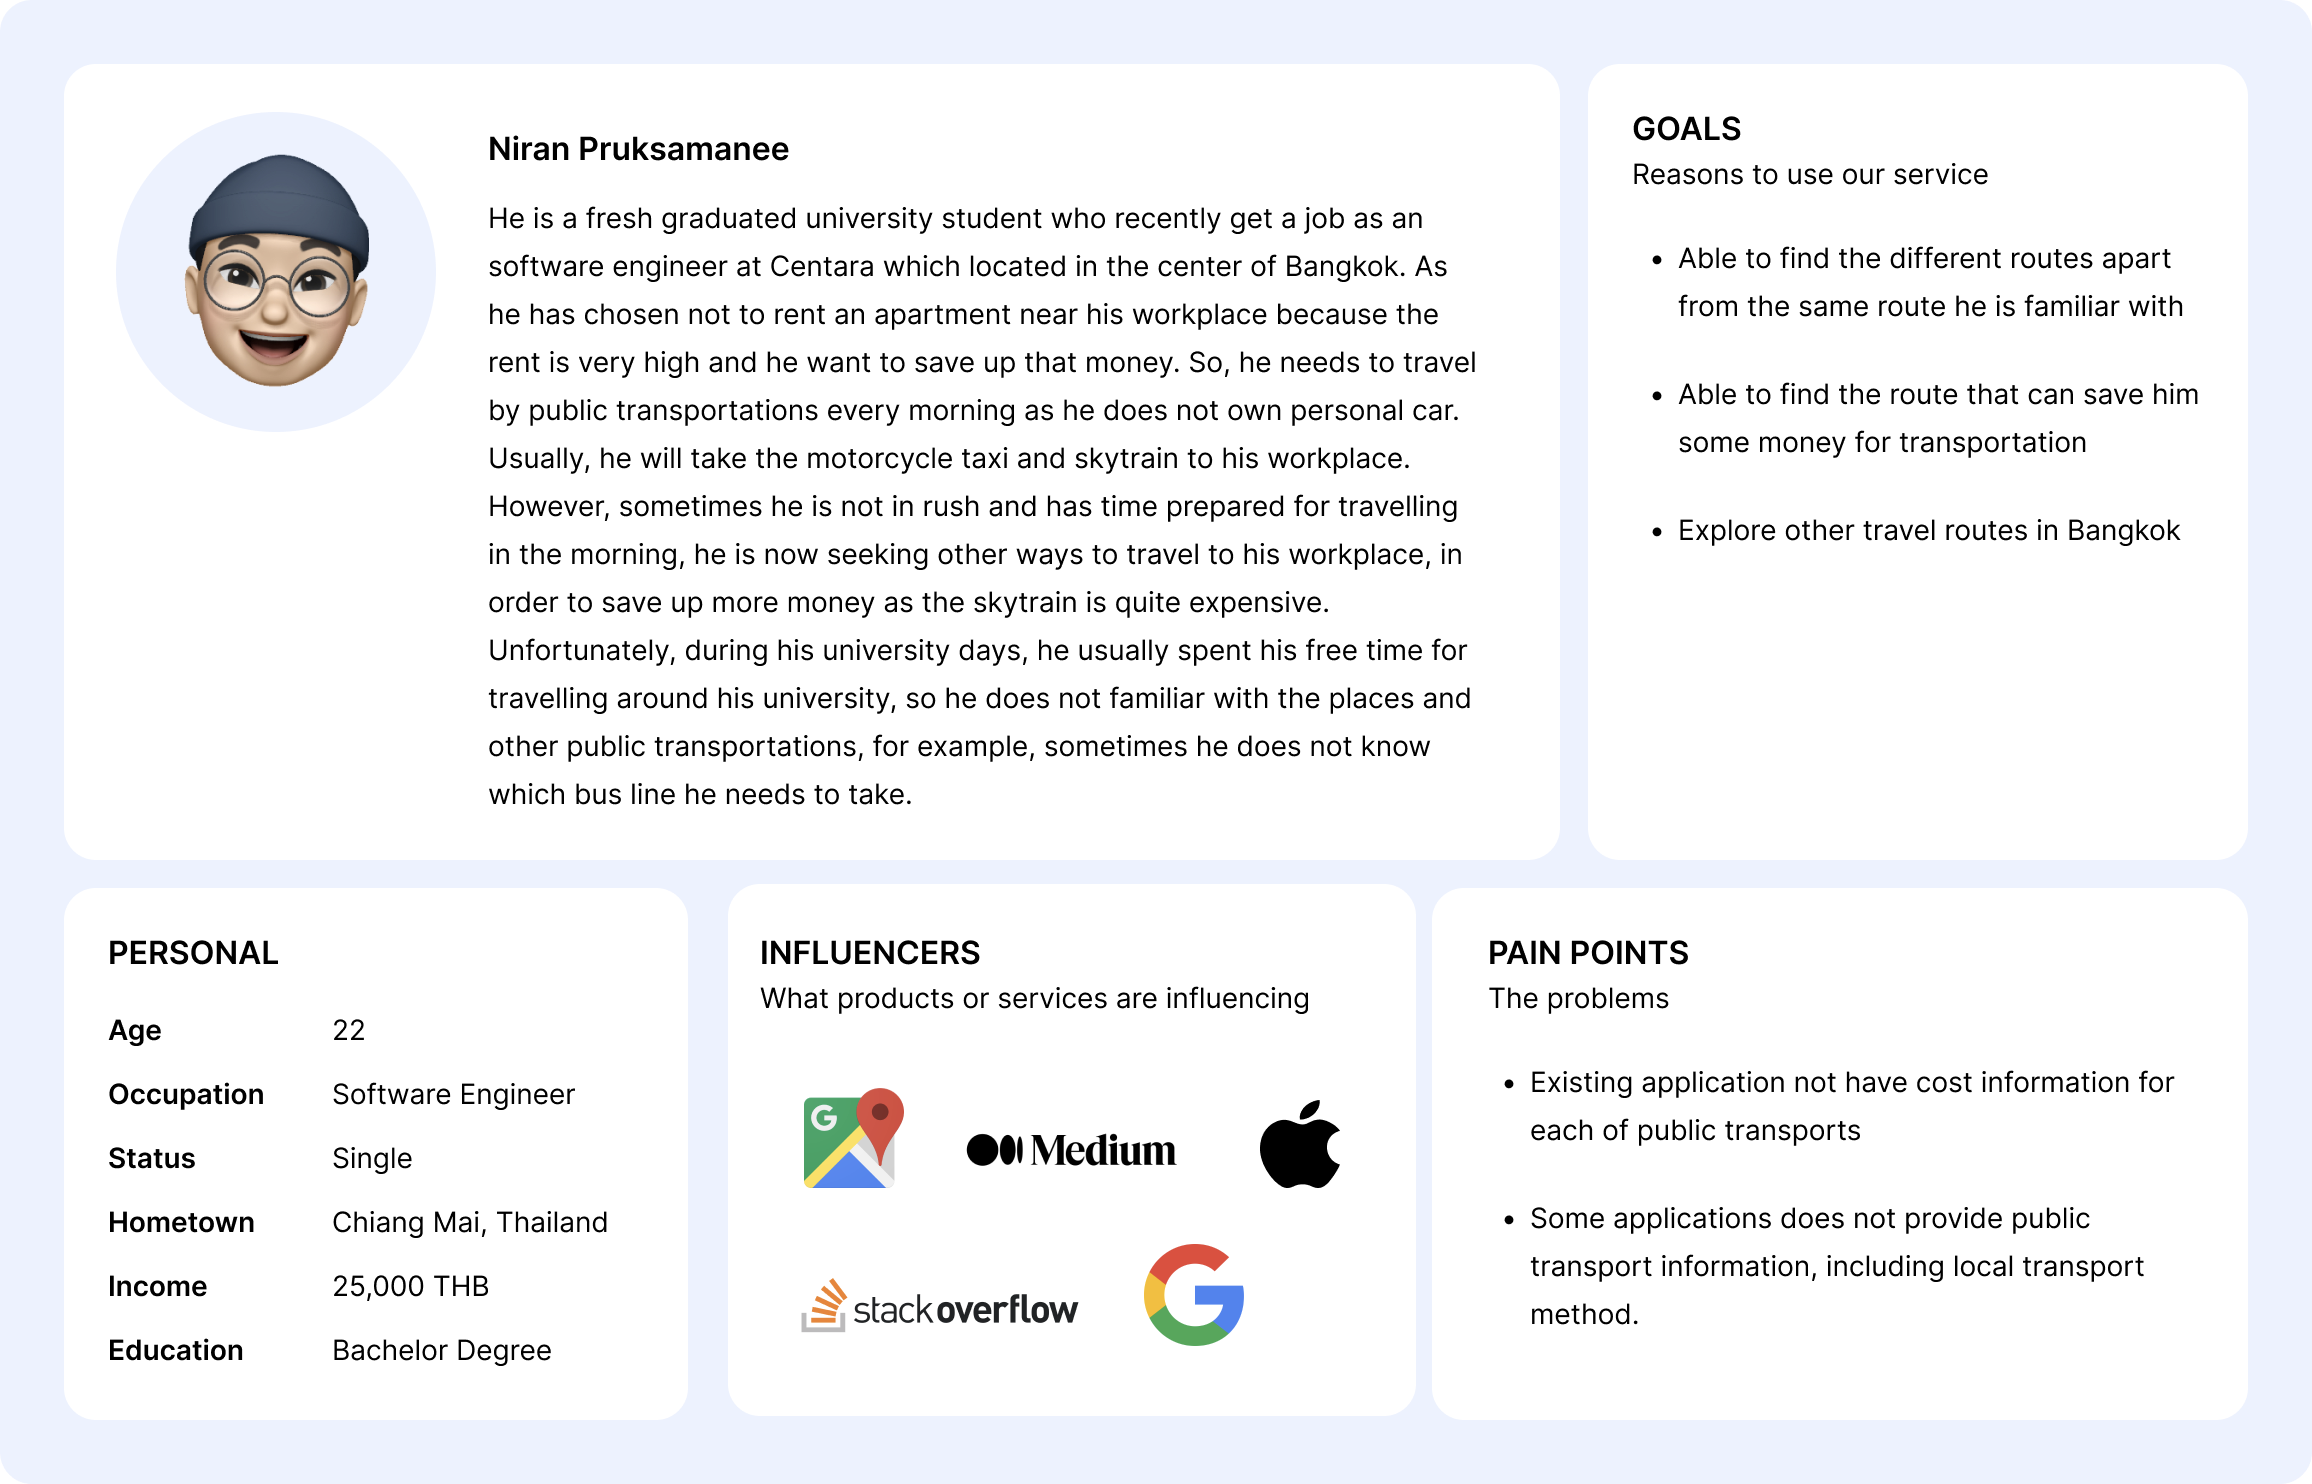
\includegraphics[width=1\linewidth]{chapter3/user-persona-3.png}
    \caption{User three persona}
    \label{fig:User three persona}
\end{figure}
\subsection{User requirement analysis}
\begin{itemize}
    \item This application helps users to find the best route for traveling.
    \item This application uses map service provider and our public transportation data such as vans, and mini truck to suggest the route for users.
    \item This application provides the community to share the routes of traveling of users.
    \item This application will provide a mobile application for users that use smartphones.
\end{itemize}

\section{Use case diagram}
\begin{figure}[!h]
    \centering
    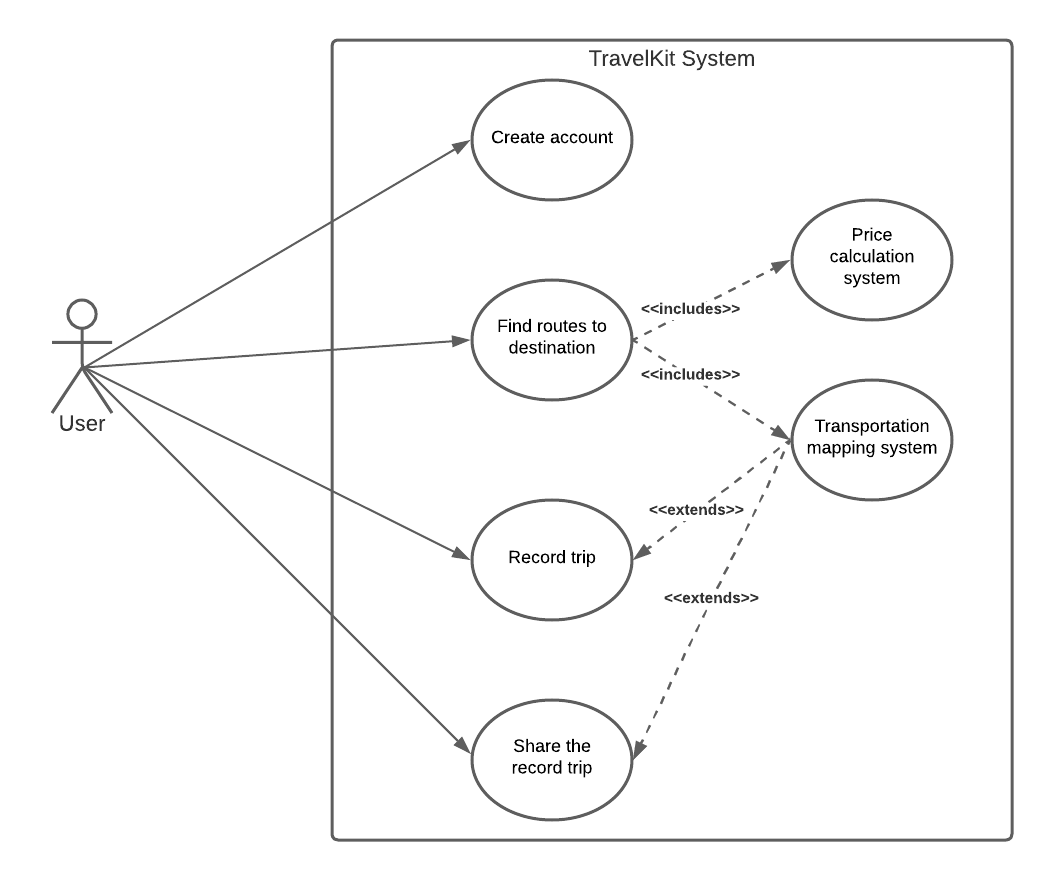
\includegraphics[width=0.7\linewidth]{chapter3/use-case-diagram.png}
    \caption{Use case diagram}
    \label{fig:Use case diagram}
\end{figure}
\par
The actor who is user in the routing system. The user must create an account to login to the system. After the user finds routes to the destination, the system will calculate the cost of traveling and display alternative routes using public transport data, such as vans and mini trucks, so that the user can make informed decisions. In addition, the user can record their trip after reaching the destination. Lastly, the user can share their trip to the community, along with the details of their travel, as well as comment and recommend other users.

\newpage
\section{Context diagram}
\begin{figure}[!h]
    \centering
    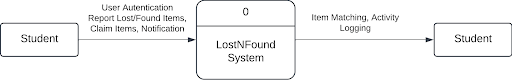
\includegraphics[width=1\linewidth]{chapter3/context-diagram.png}
    \caption{Context diagram}
    \label{fig:Context diagram}
\end{figure}
\par
The context diagram shows the overall of the TravelKit system that required the name, password, user’s location, destination. Then, the system will create choices of the routes, directions and calculate the cost of traveling to the destination.

\section{Activity diagram}
\subsection{Travel process}
\begin{figure}[!h]
    \centering
    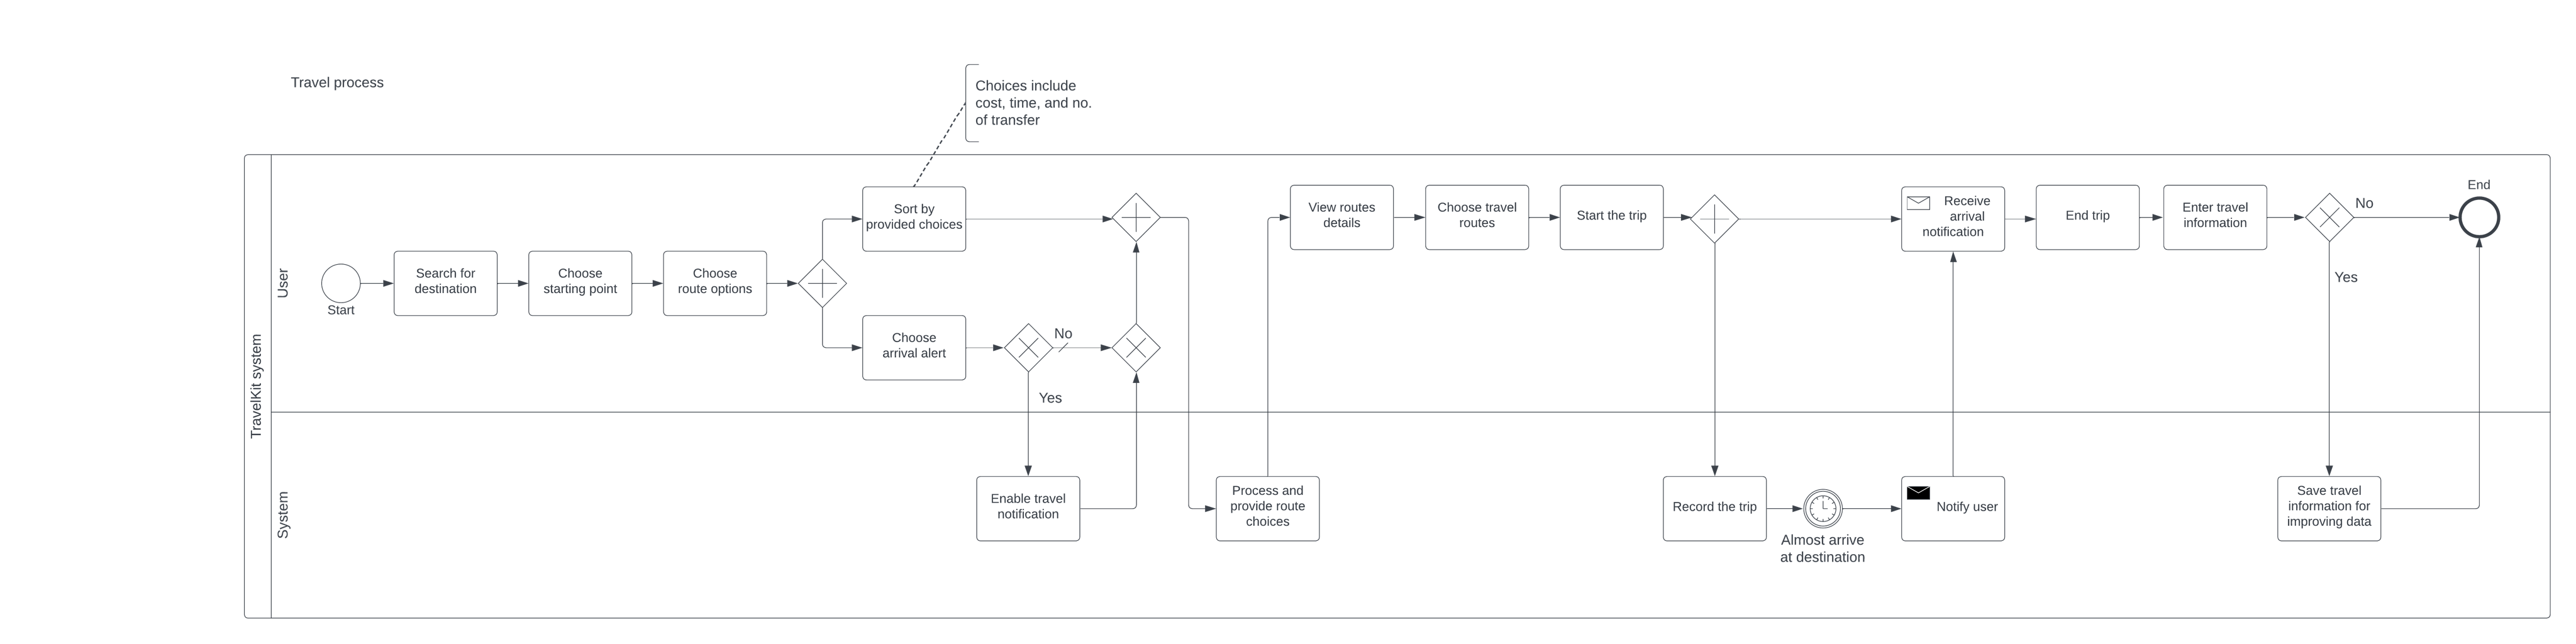
\includegraphics[width=1\linewidth]{chapter3/travel-process.png}
    \caption{Travel process}
    \label{fig:Travel process}
\end{figure}
\par
The travel process for the TravelKit system starts when the user searches for the designated destination. Then, the user will be presented with the default starting point, which the user can either use their current location or select it again. After that, the user will choose their route options, which include the travel cost, time, number of transfers, and the arrival alert. If the user desires to have an arrival alert, the system will enable travel notification. Subsequently, the user can see the provided routes details, choose the route and then start the trip. Meanwhile, the system will start recording the trip and send the notification to the user when they are almost arriving at the destination. Finally, the user can choose either to share their travel route or not. If they choose to do so, the system will save the travel information to improve our system data and user can share to other people in community.

\newpage
\subsection{Community process}
\begin{figure}[!h]
    \centering
    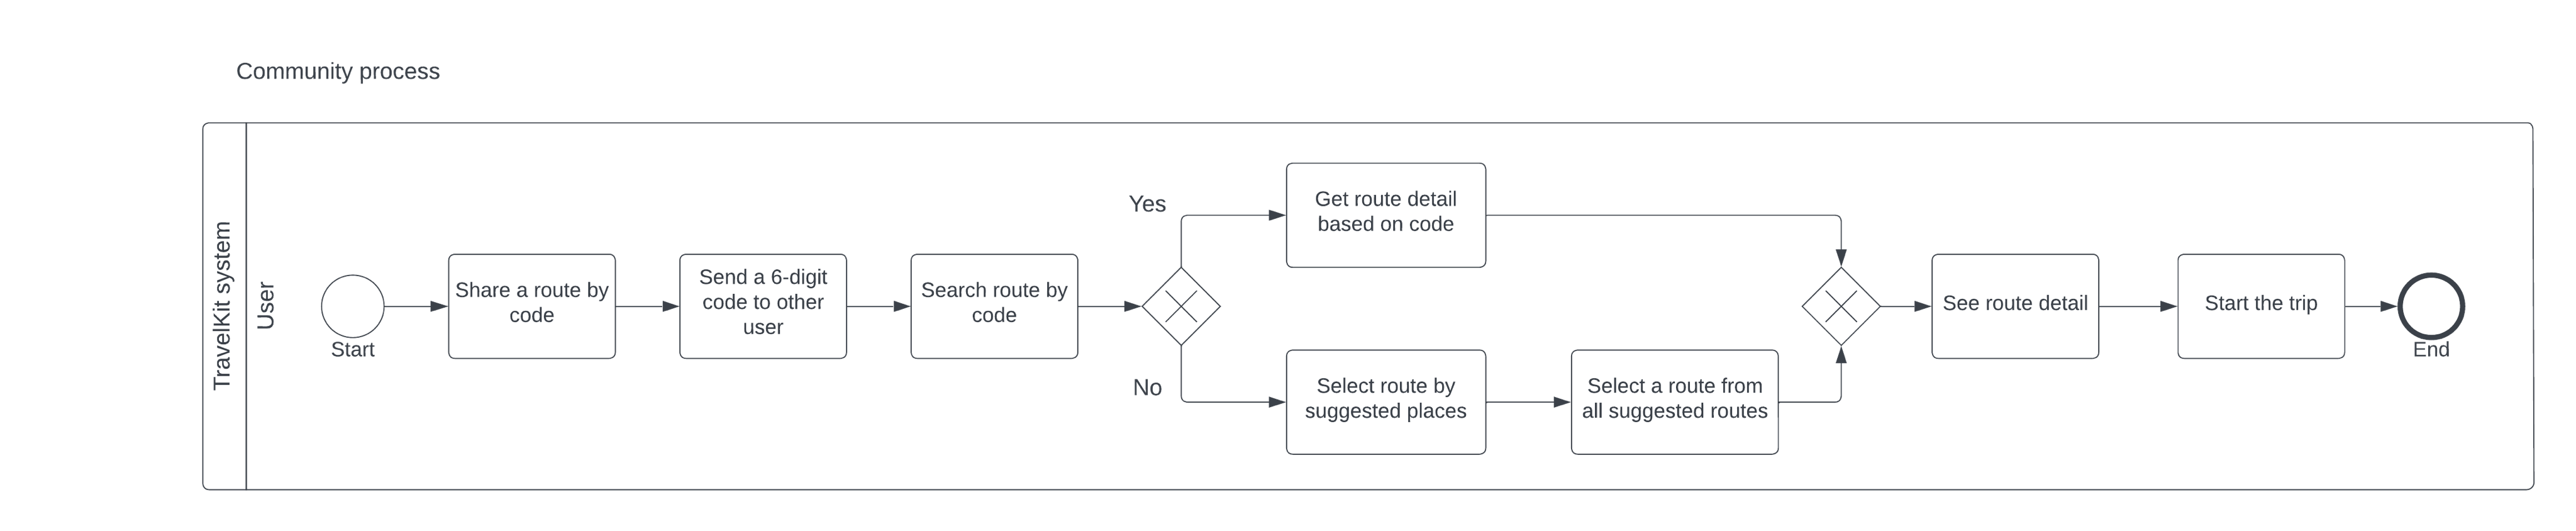
\includegraphics[width=1\linewidth]{chapter3/community-process.png}
    \caption{Community process}
    \label{fig:Community process}
\end{figure}
\par
The community processes for the TravelKit system can be divided into two sub-processes. The first process is for the users who desire to search for routes, which can enter the code to get exact route detail. The second process is for users who wish to find for routes or  places recommendations. The process starts when the user select the destination. Afterwards, the user can view the recommended routes and then select the route they preferred.

\newpage
\section{Database design}
\subsection{Relational Database}
\begin{figure}[!h]
	\centering
	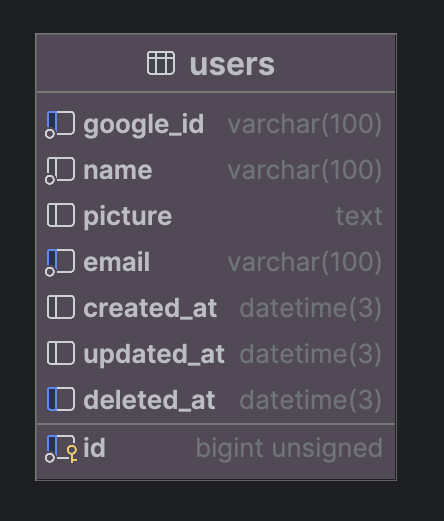
\includegraphics[width=0.5\linewidth]{chapter3/sql-db-schema.png}
	\caption{Relational Database Schema}
	\label{fig:Relational Database Schema}
\end{figure}
Our database relies on MySQL to store user data efficiently. It is intricately connected with MongoDB, particularly in managing community-related information. This dual-database approach enhances functionality, ensuring seamless integration between individual user data and community features, contributing to a robust and scalable system.

\newpage
\subsection{non-relational database}
\begin{figure}[!h]
    \centering
    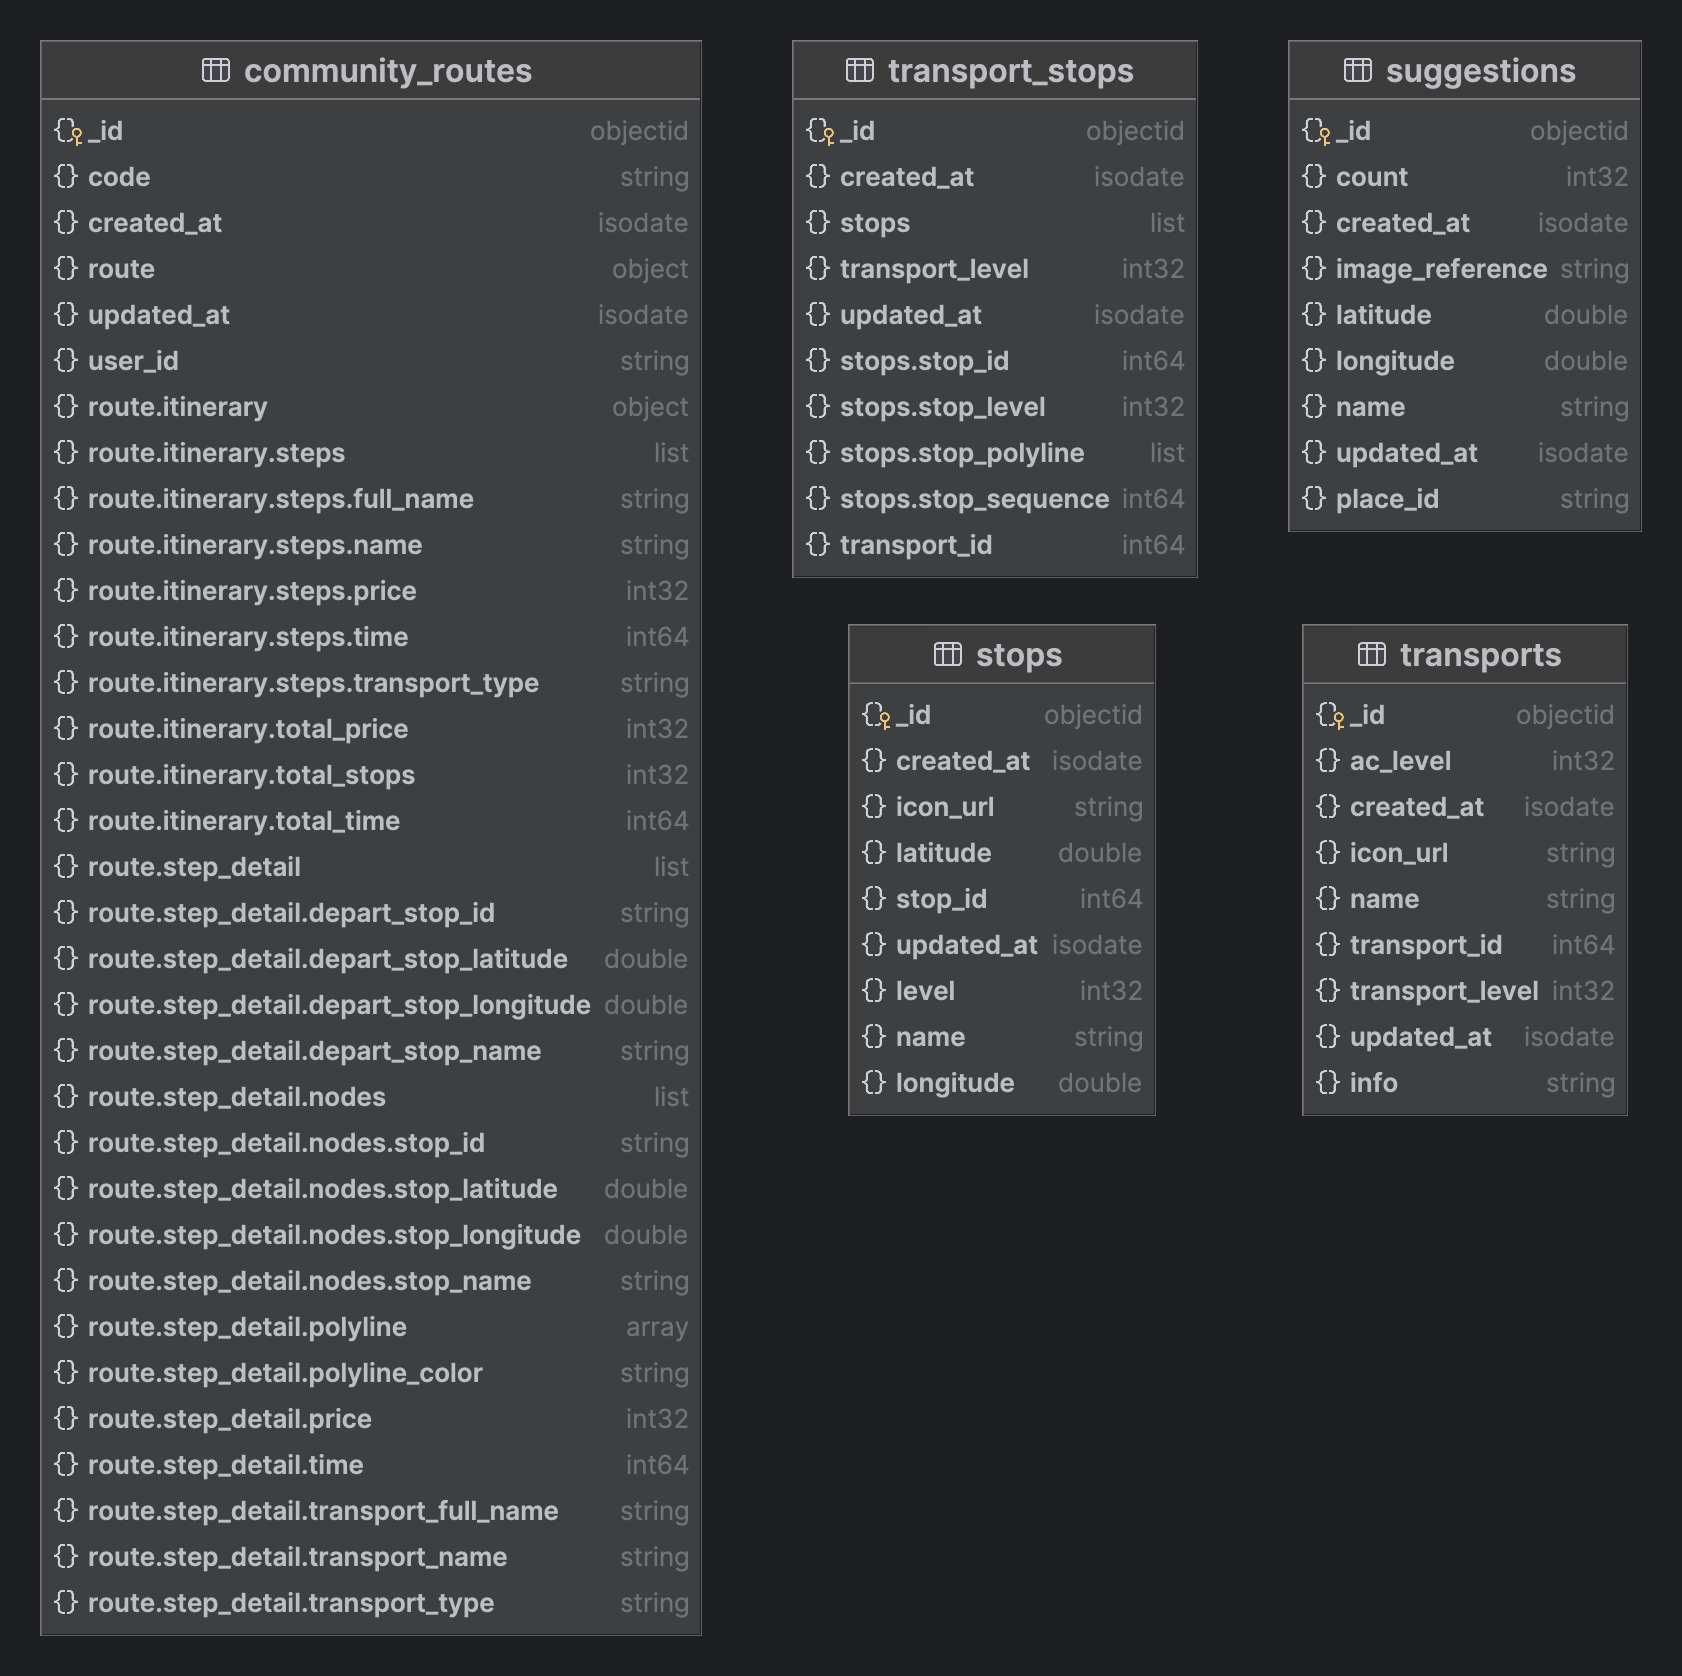
\includegraphics[width=0.6\linewidth]{chapter3/nosql-db-schema.png}
    \caption{Non-Relational Database Schema}
    \label{fig:Non-Relational Database Schema}
\end{figure}
MongoDB is used for storing transport data, stops, and each stop related to each route. It includes:
\begin{itemize}
	\item \textbf{Transports} for storing all data about transport types and transports
	\item \textbf{Stops} for storing stop data, such as bus stops, train stations, and ports
	\item \textbf{Transport Stops} for storing all stops that relate to each transport sequentially
	\item \textbf{Community Routes} for storing shared routes from each users
	\item \textbf{Suggestion} for storing the most frequently selected destinations by users
\end{itemize}

\newpage
\subsection{Graph Database}
The graph database used for storing routes and stops relationship for using the algorithm to find shortest path based on user queries. The graph consist of nodes and relations which is the following node types:
\begin{itemize}
	\item \textbf{STOP} For storing stop or station of all transportation type (e.g. National Theatre, Sanam Luang Bus Terminal, Hua Lamphong, Opposite Tha Phra Chan)
	\item \textbf{ARL} For each line of Airport Rail Link system
	\item \textbf{BRT} For each line of Bus Rapid Transit system
	\item \textbf{BTS} For each line of BTS Skytrain system
	\item \textbf{BUS} For each route of BMTA bus line
	\item \textbf{CHE} For each route of Chao Phraya Express Boat
	\item \textbf{KPS} For each route of minibus and local mini truck
	\item \textbf{MRT} For each line of Metropolitan Rapid Transit
	\item \textbf{SRT} For each line of train
\end{itemize}
\par
Concerning relationships, the project incorporates various types tailored for tasks such as shortest path finding  \cite{neo4j2}, performance optimization, and conditional querying. These relationships are categorized as follows:

\newpage
\subsubsection{GOTO relationship}
\begin{figure}[!h]
	\centering
	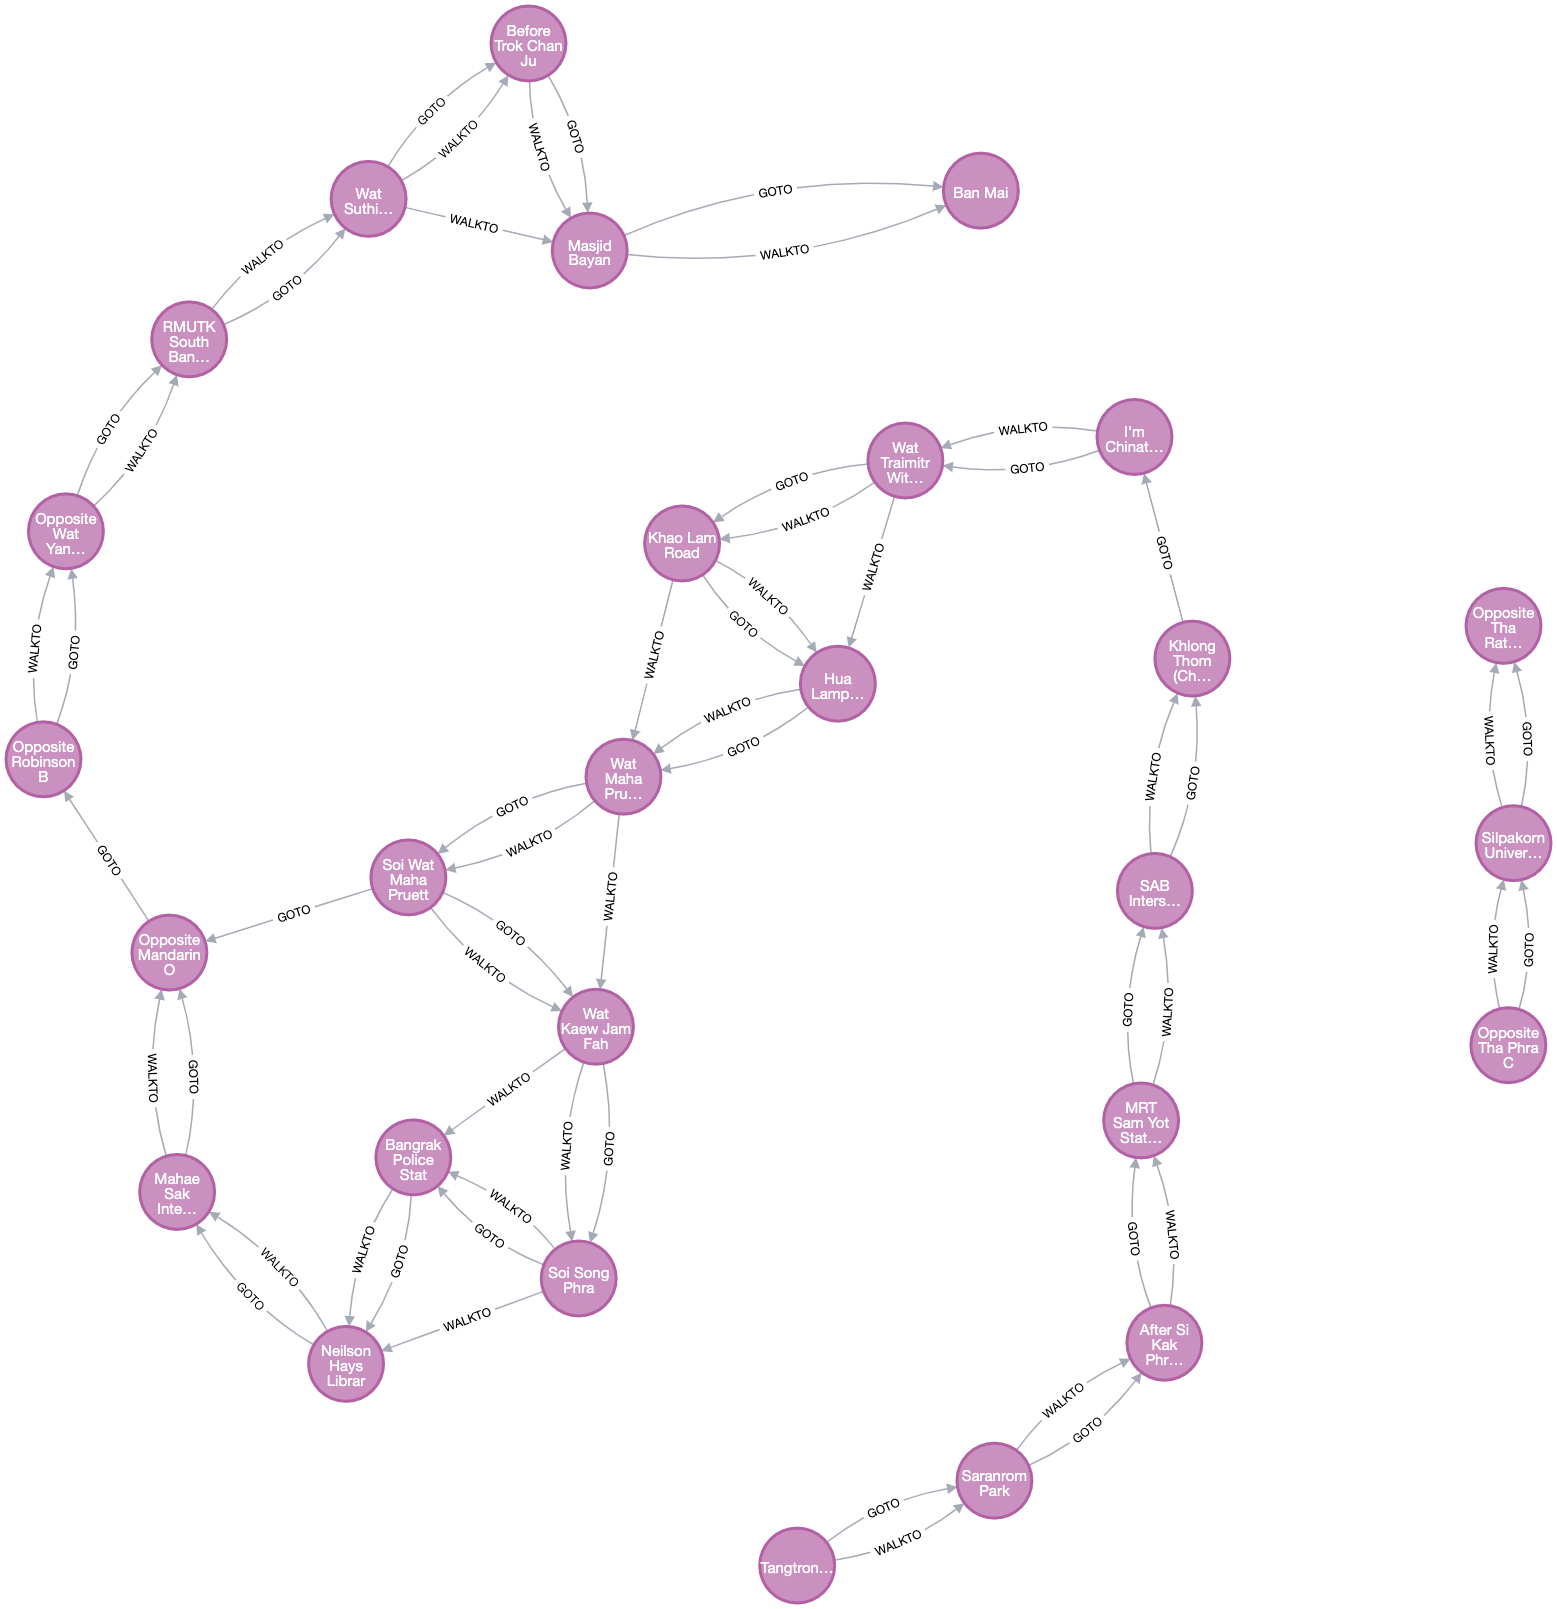
\includegraphics[width=1\linewidth]{chapter3/goto_relationship.png}
	\caption{GOTO relationship}
	\label{fig:GOTO relationship}
\end{figure}
The relation of each two stops that are next to each other and have at least one transportation that pass from one to another (for example, from Sanam Luang stop to National Theatre stop) consider as one-way direction of each side of the road. This relation used for specifying the stop that are available for each bus line to transfer to another

\newpage
\subsubsection{WALKTO relationship}
\begin{figure}[!h]
	\centering
	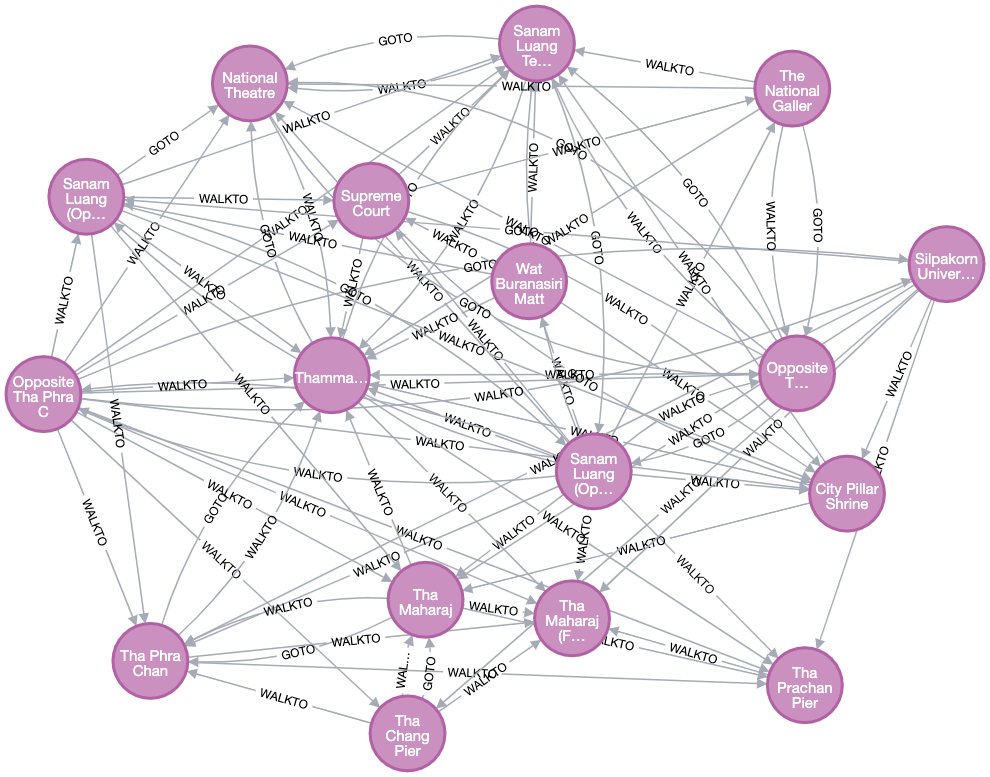
\includegraphics[width=1\linewidth]{chapter3/walkto_relationship.png}
	\caption{WALKTO relationship}
	\label{fig:WALKTO relationship}
\end{figure}
As GOTO relation might not enough for finding the best suitable route, since some stops may not next to each other but user can transfer, walk or reroute between bus line that are in opposite direction for shorter distance. So we create WALKTO relation for all pair of stops that are walkable within 500 meters for querying the route which user can transfer to the nearby stop which are not directly next to each other.

\newpage
\subsubsection{STOPAT/STOPBY relationship}
\begin{figure}[!h]
	\centering
	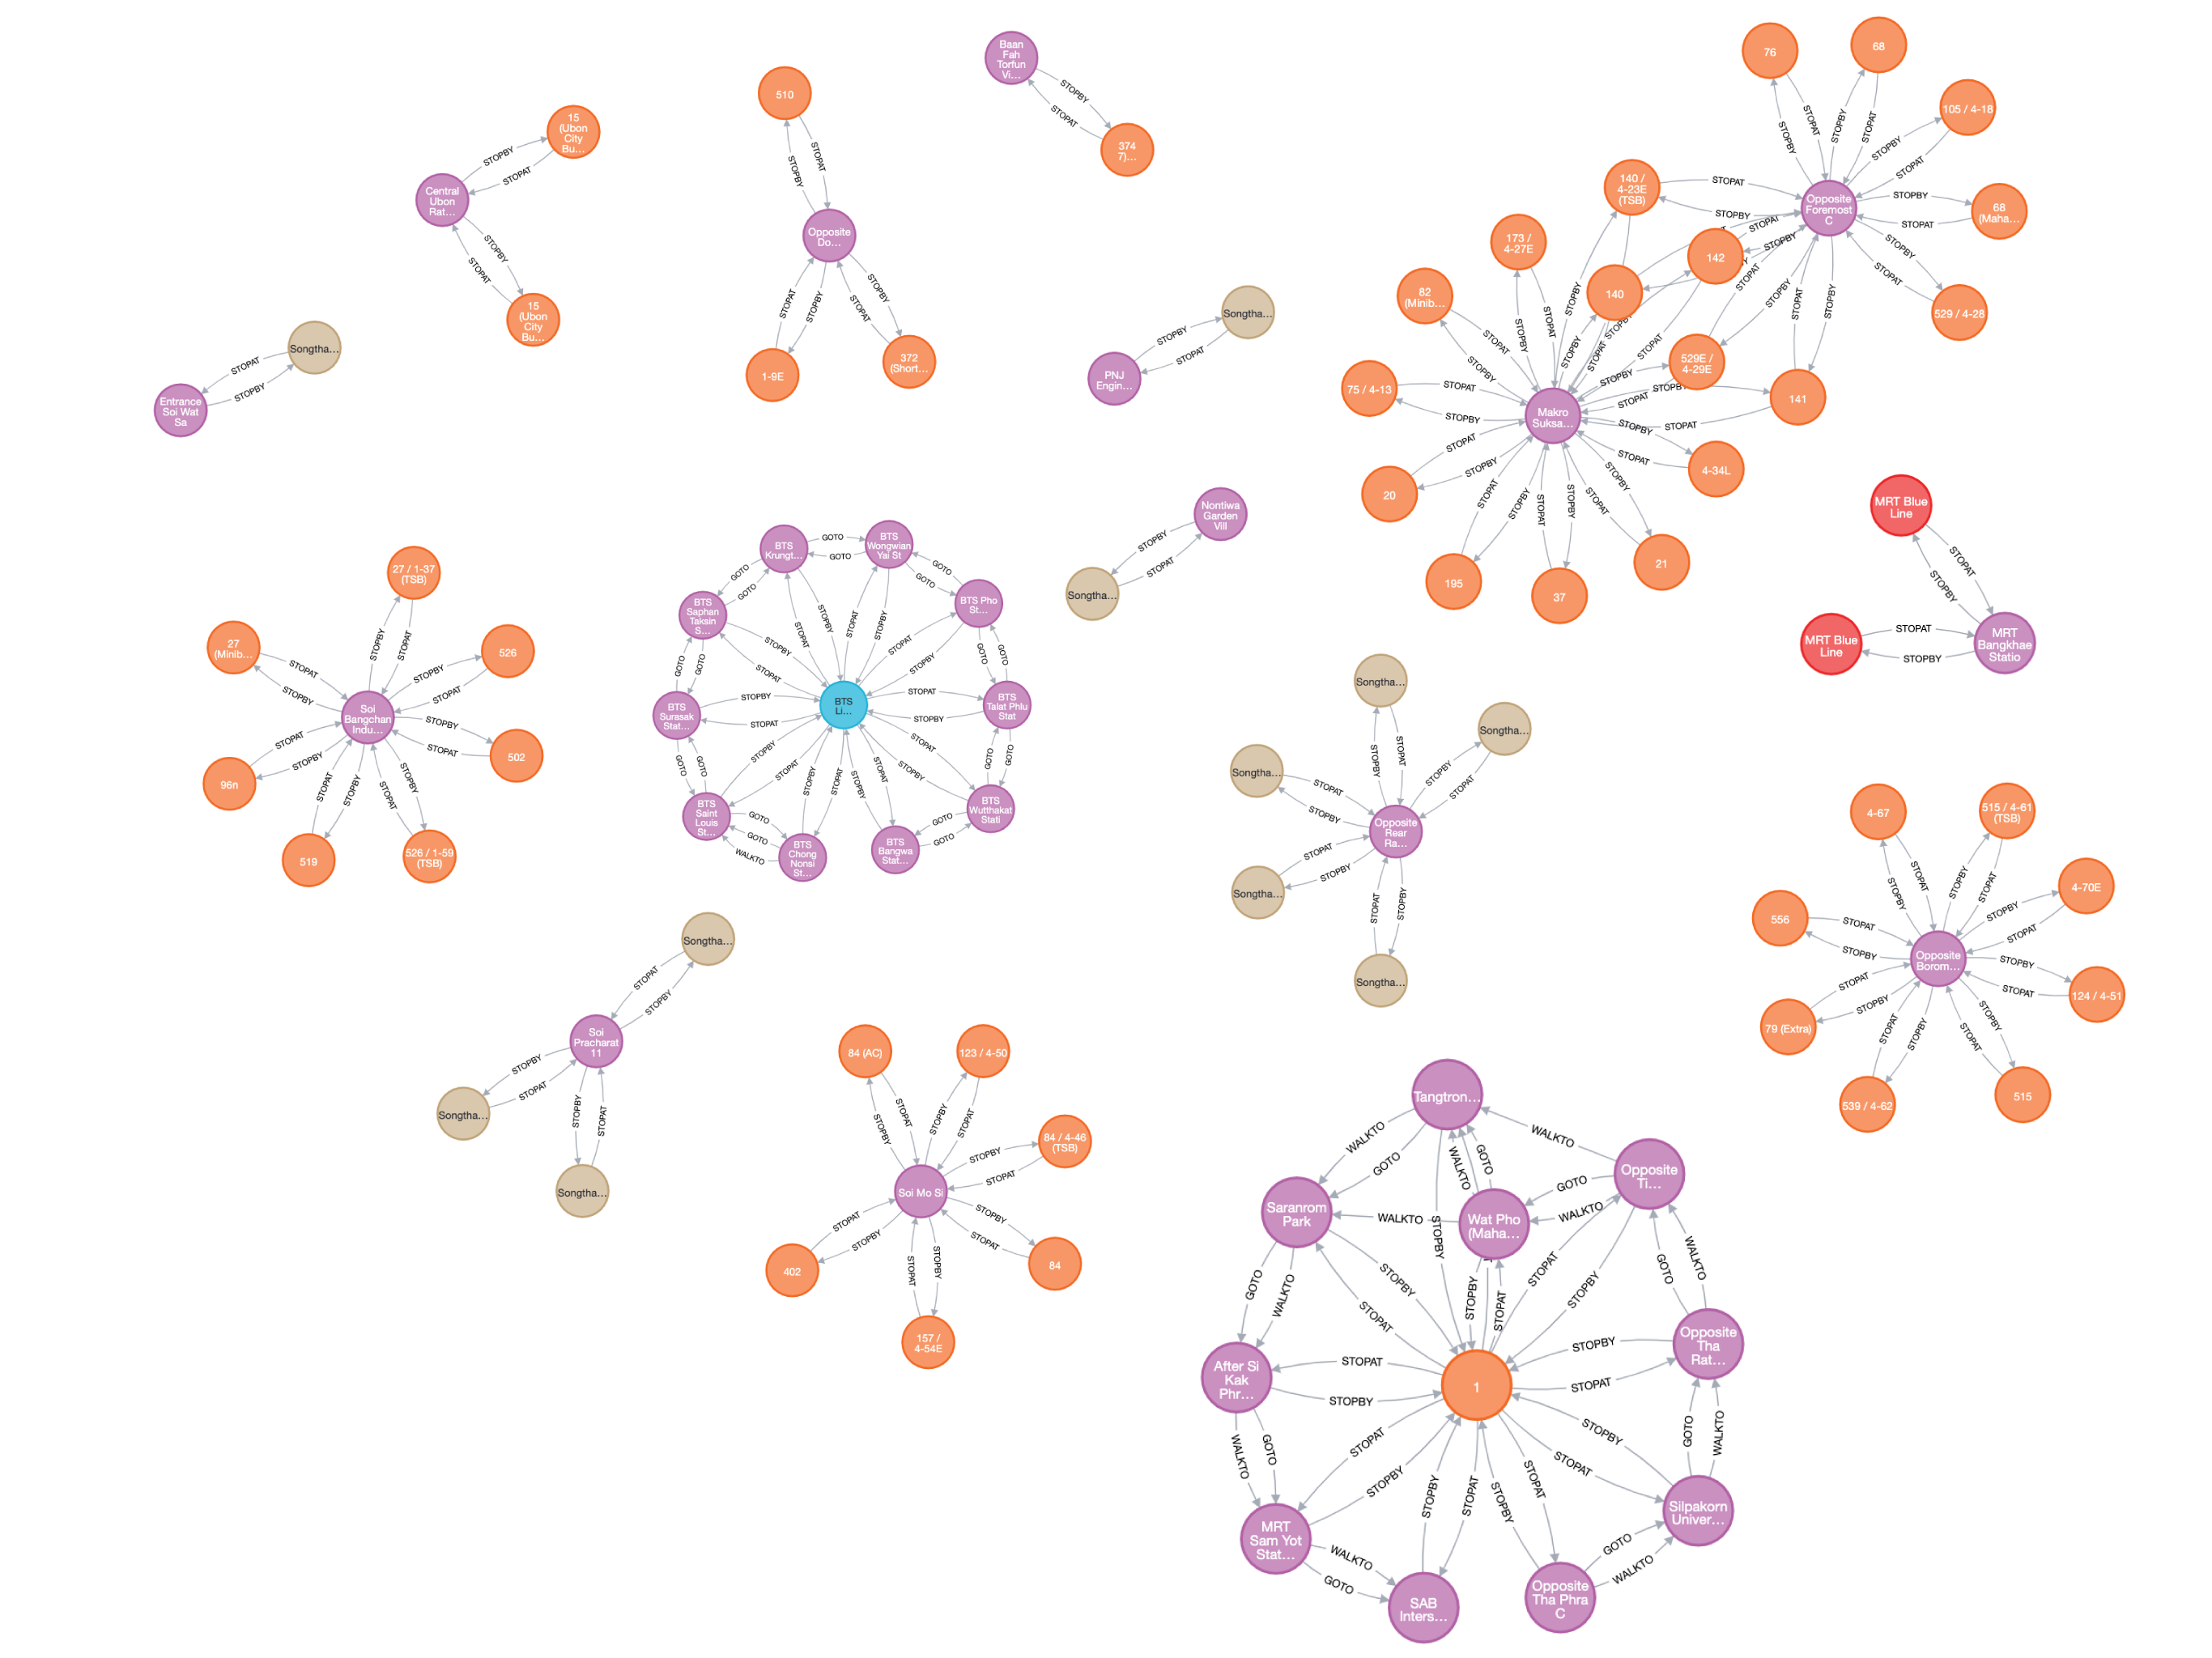
\includegraphics[width=1\linewidth]{chapter3/stopat_relationship.png}
	\caption{STOPAT/STOPBY relationship}
	\label{fig:STOPAT/STOPBY relationship}
\end{figure}
The relationship represent that each transportation line (e.g., bus line, BTS line) are stop at each stop/stations. Each stop are stoppable from many transportation line and each transportation line can pass trough and stoppable at many stop as well.
\chapter{System functionality}
\section{Introduction}
This chapter describes the core aspects of the system's functionality, covering its system architecture, primary functions, planning, and testing results that defined the application's capabilities. The first part covers the architecture of the system in this project and the second part covers the main functionality of the system.
\section{System architecture}

\begin{figure}[!h]
    \centering
    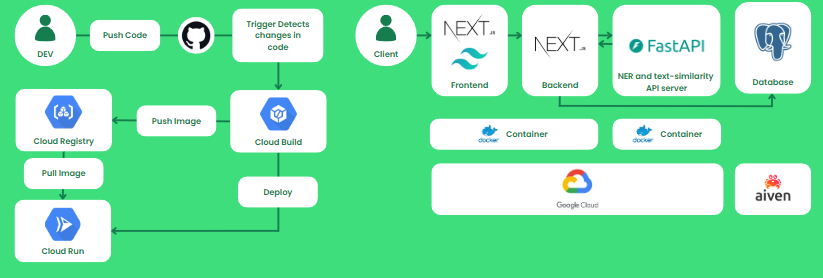
\includegraphics[width=1\linewidth]{chapter4/sysarch.png}
    \caption{System architecture}
    \label{fig:System architecture}
\end{figure}
The system will consist of two main components. The first component is frontend, the user-interaction part written as Flutter application which has functionalities of login, using Google OAuth API and has the map preview for user to search for places and navigate through routes. It will have to retrieve raw location data from the device GPS and call to backend using REST API. The second component is backend, which consists of the data manipulation and algorithmic part, which written using Golang. The backend use for retrieve route request from frontend, then All the connections between frontend and backend are proxies trough Cloudflare and internal NGINX reverse proxy. For the backend process, we use MariaDB for relational data store, Neo4j \cite{neo4j} for graph data store, The maps library, Google Maps API and self-hosted OSRM API, is used gather places, routes and any geographic information.

\section{Main function}
\begin{figure}[!h]
	\centering
	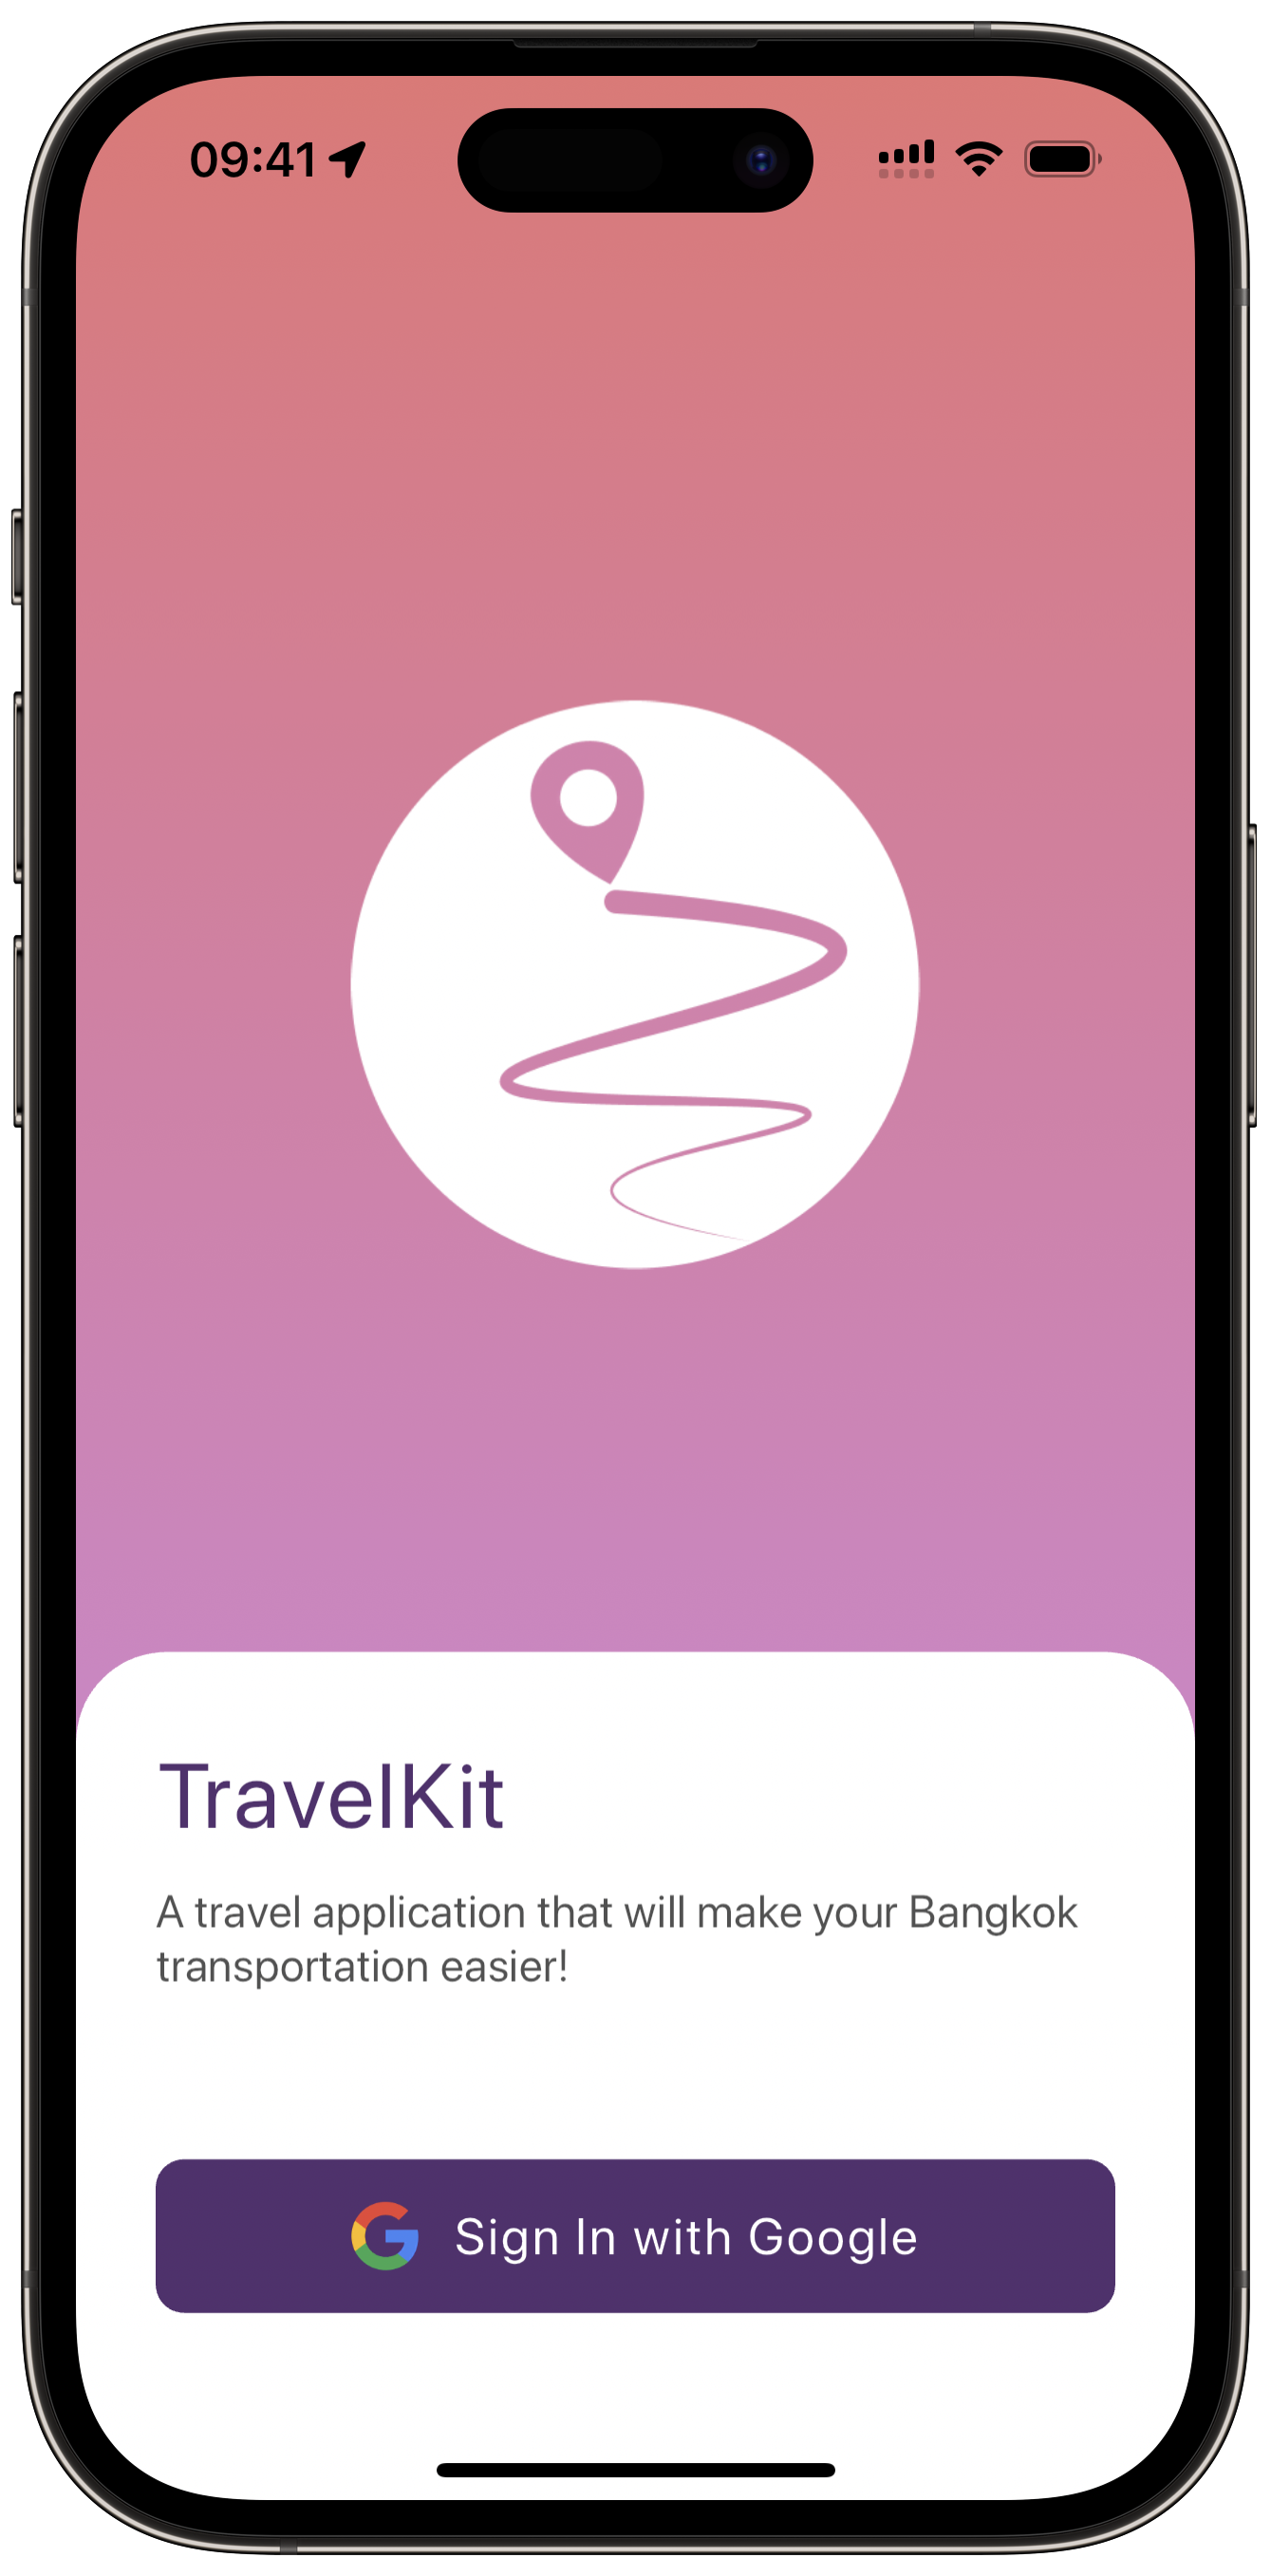
\includegraphics[width=0.5\linewidth]{chapter4/welcome_screen.png}
	\caption{Welcome screen}
	\label{fig:Welcome screen}
\end{figure}
This figure shows the welcome message and login button, Users can log in by Google to register and log into our application.

\newpage
\begin{figure}[!h]
	\centering
	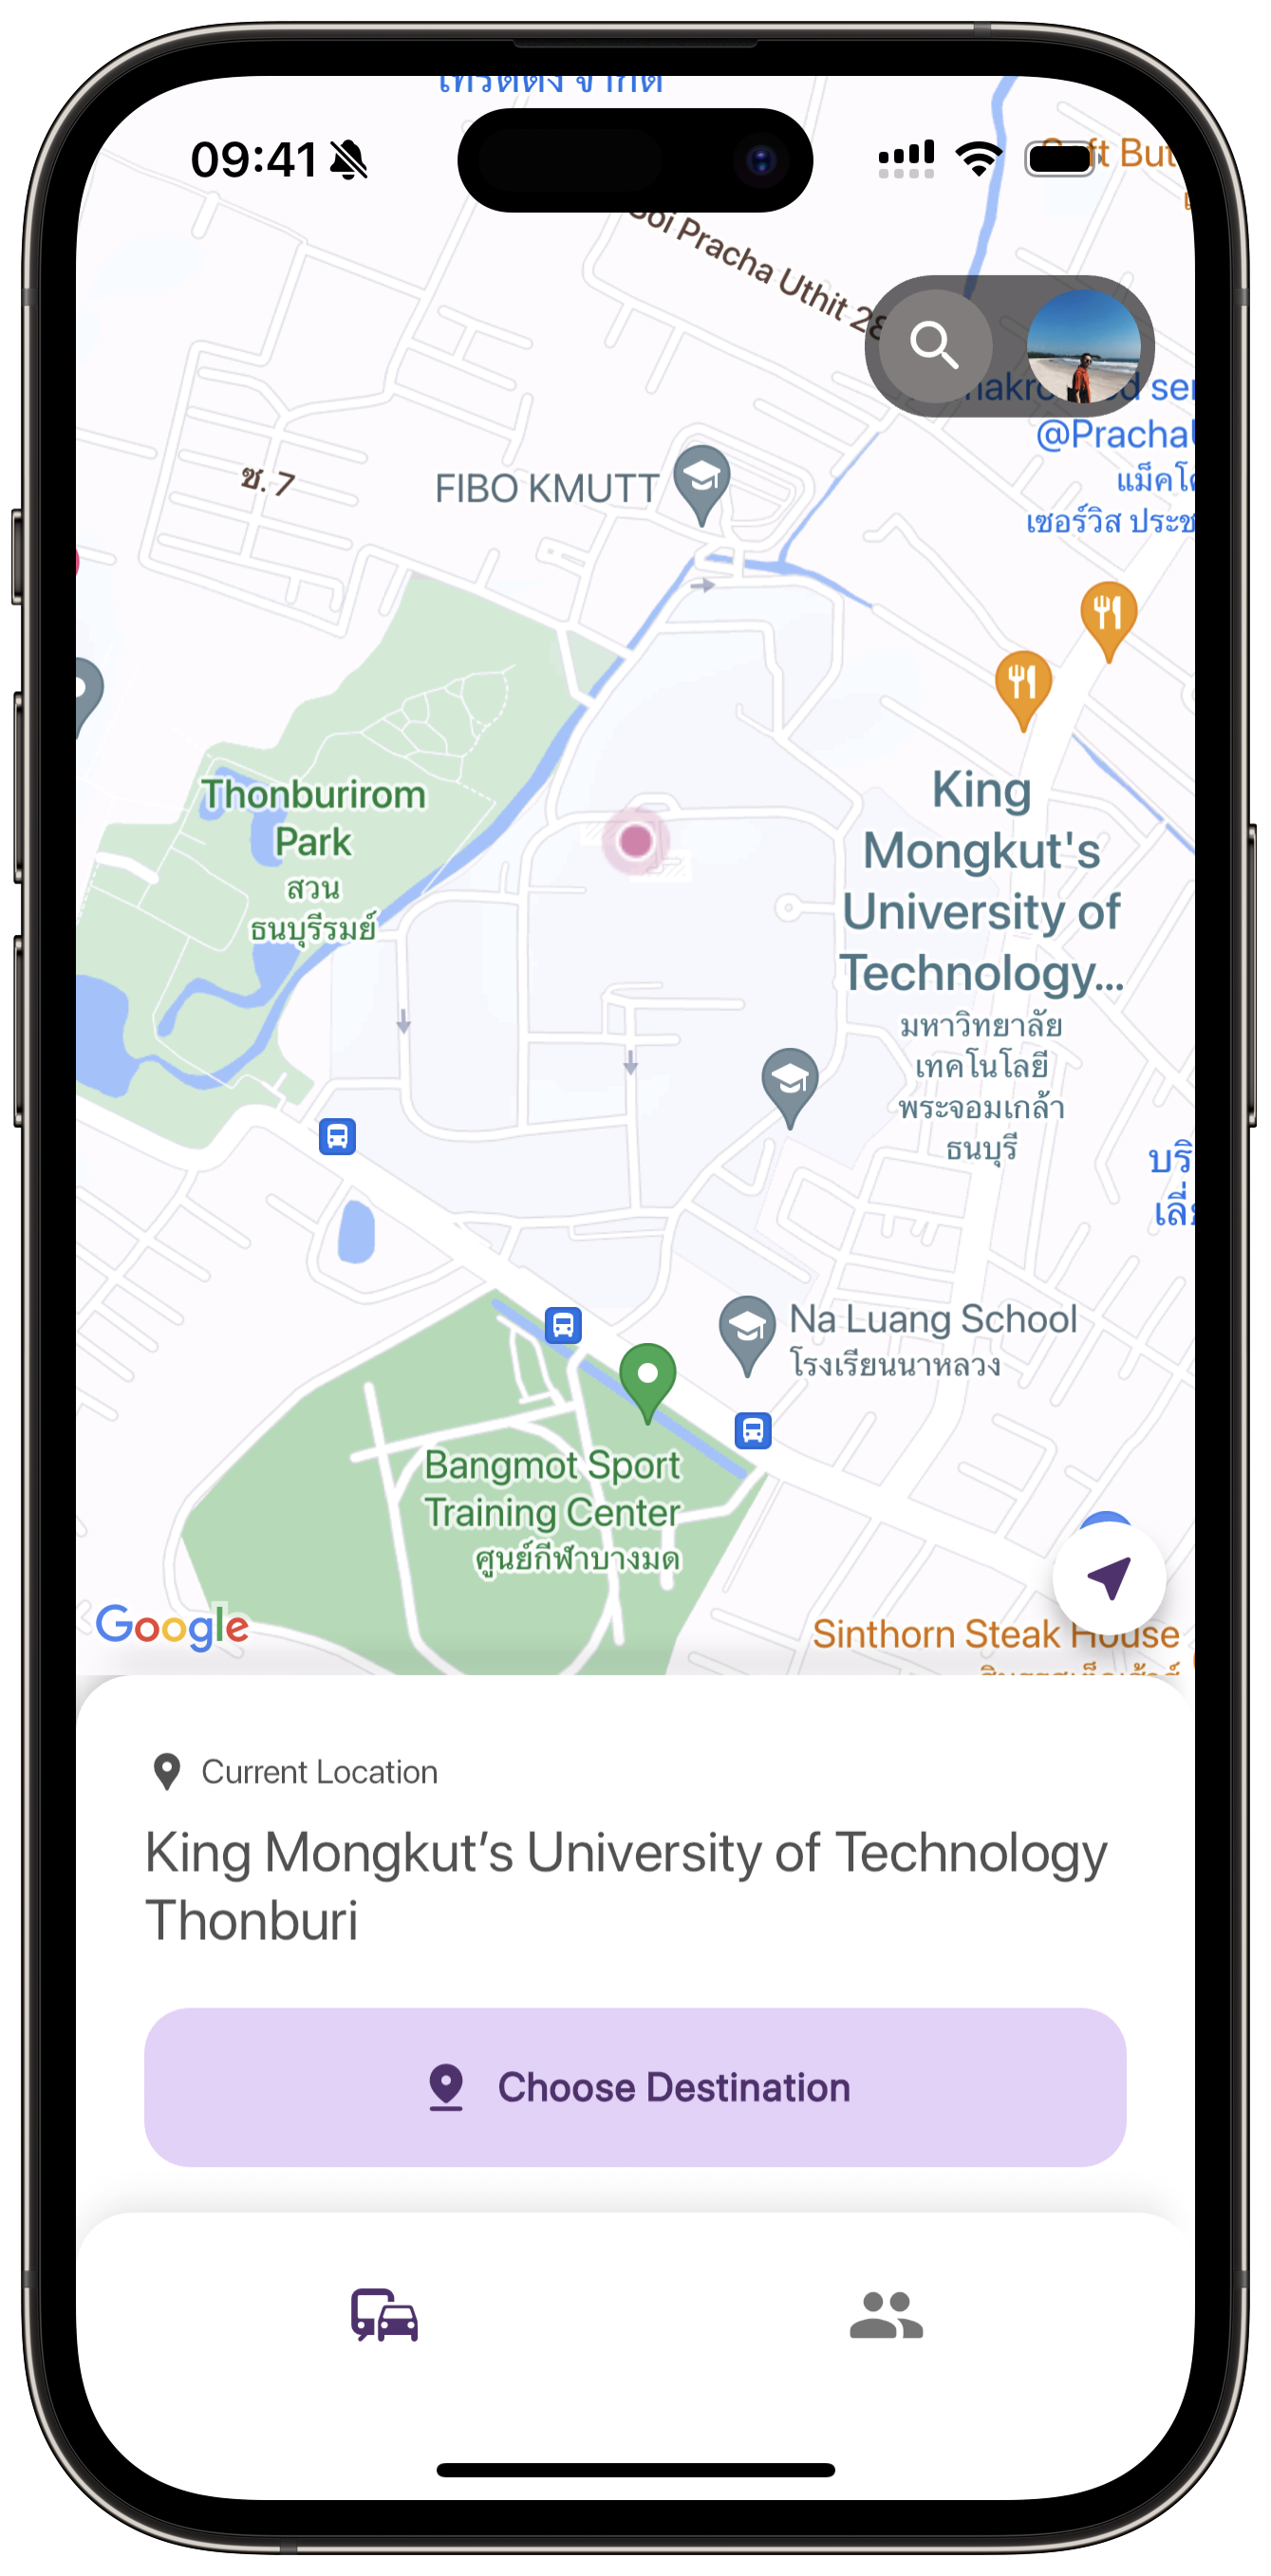
\includegraphics[width=0.5\linewidth]{chapter4/home_screen.png}
	\caption{Home screen}
	\label{fig:Home screen}
\end{figure}
This figure shows the map, current location, the name the current location after logging in and the user can tap the location icon to update the map screen to show their current location. The user can switch between the home screen and the community screen using the bottom navigation bar below.

\newpage
\begin{figure}[!h]
	\centering
	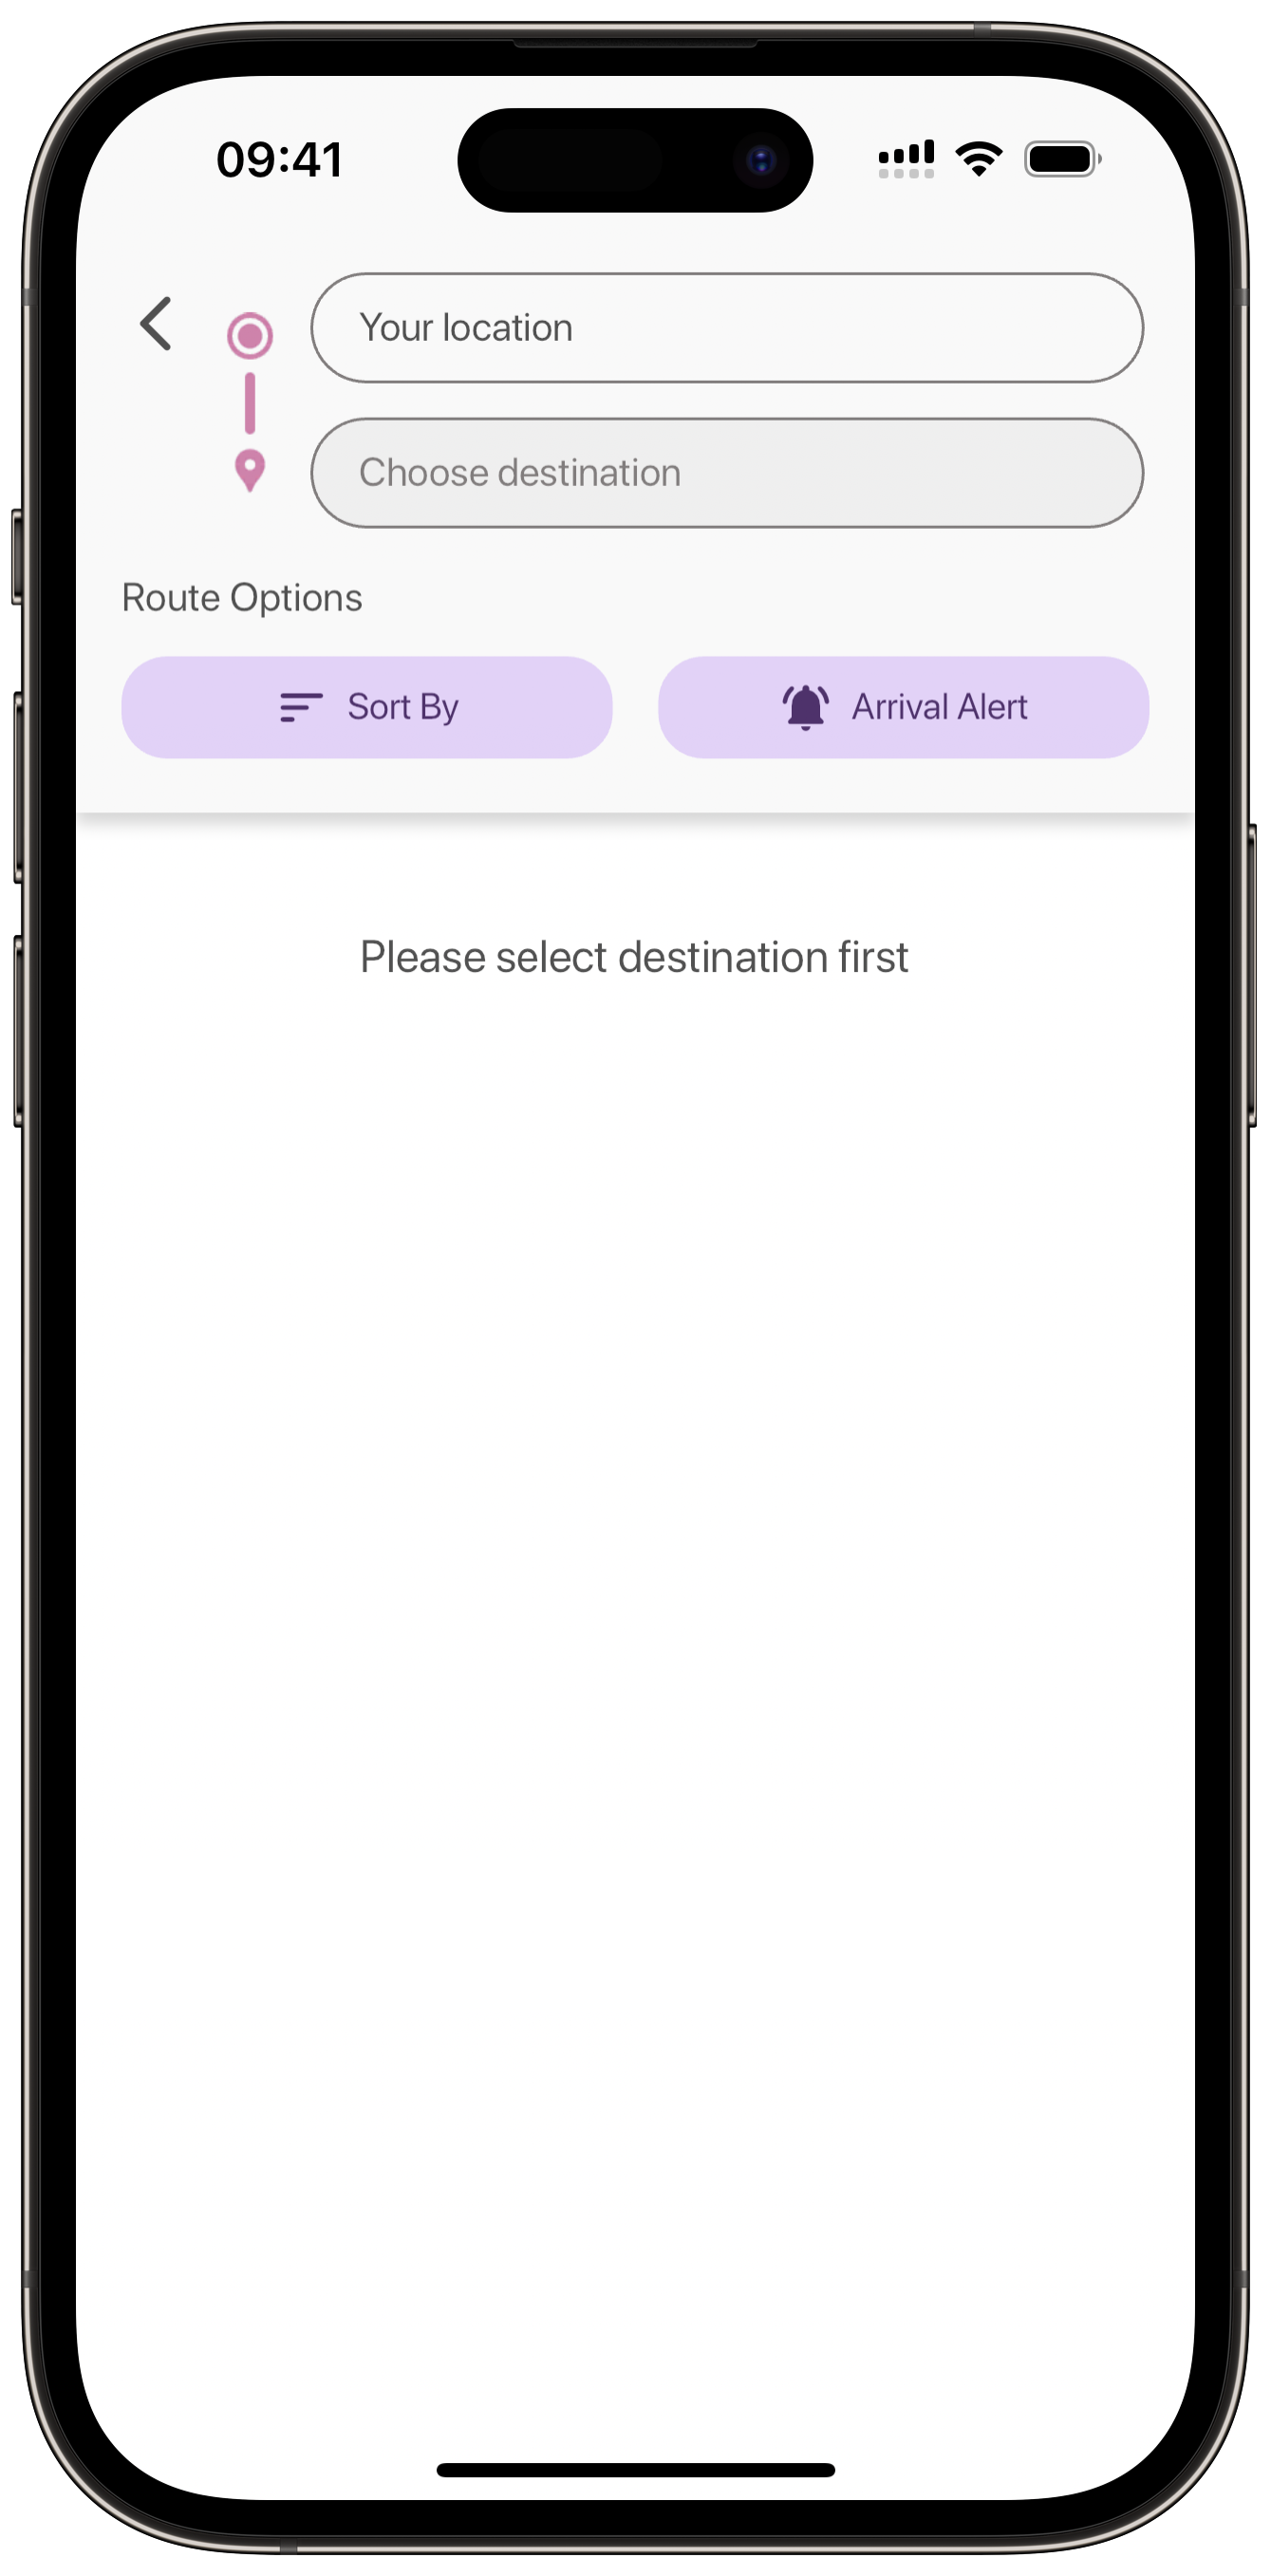
\includegraphics[width=0.5\linewidth]{chapter4/choosing_destination_screen.png}
	\caption{Choosing destination screen}
	\label{fig:Choosing destination screen}
\end{figure}
Users can search routes by specifying both the starting location and the destination to find routes for users.

\newpage
\begin{figure}[!h]
	\centering
	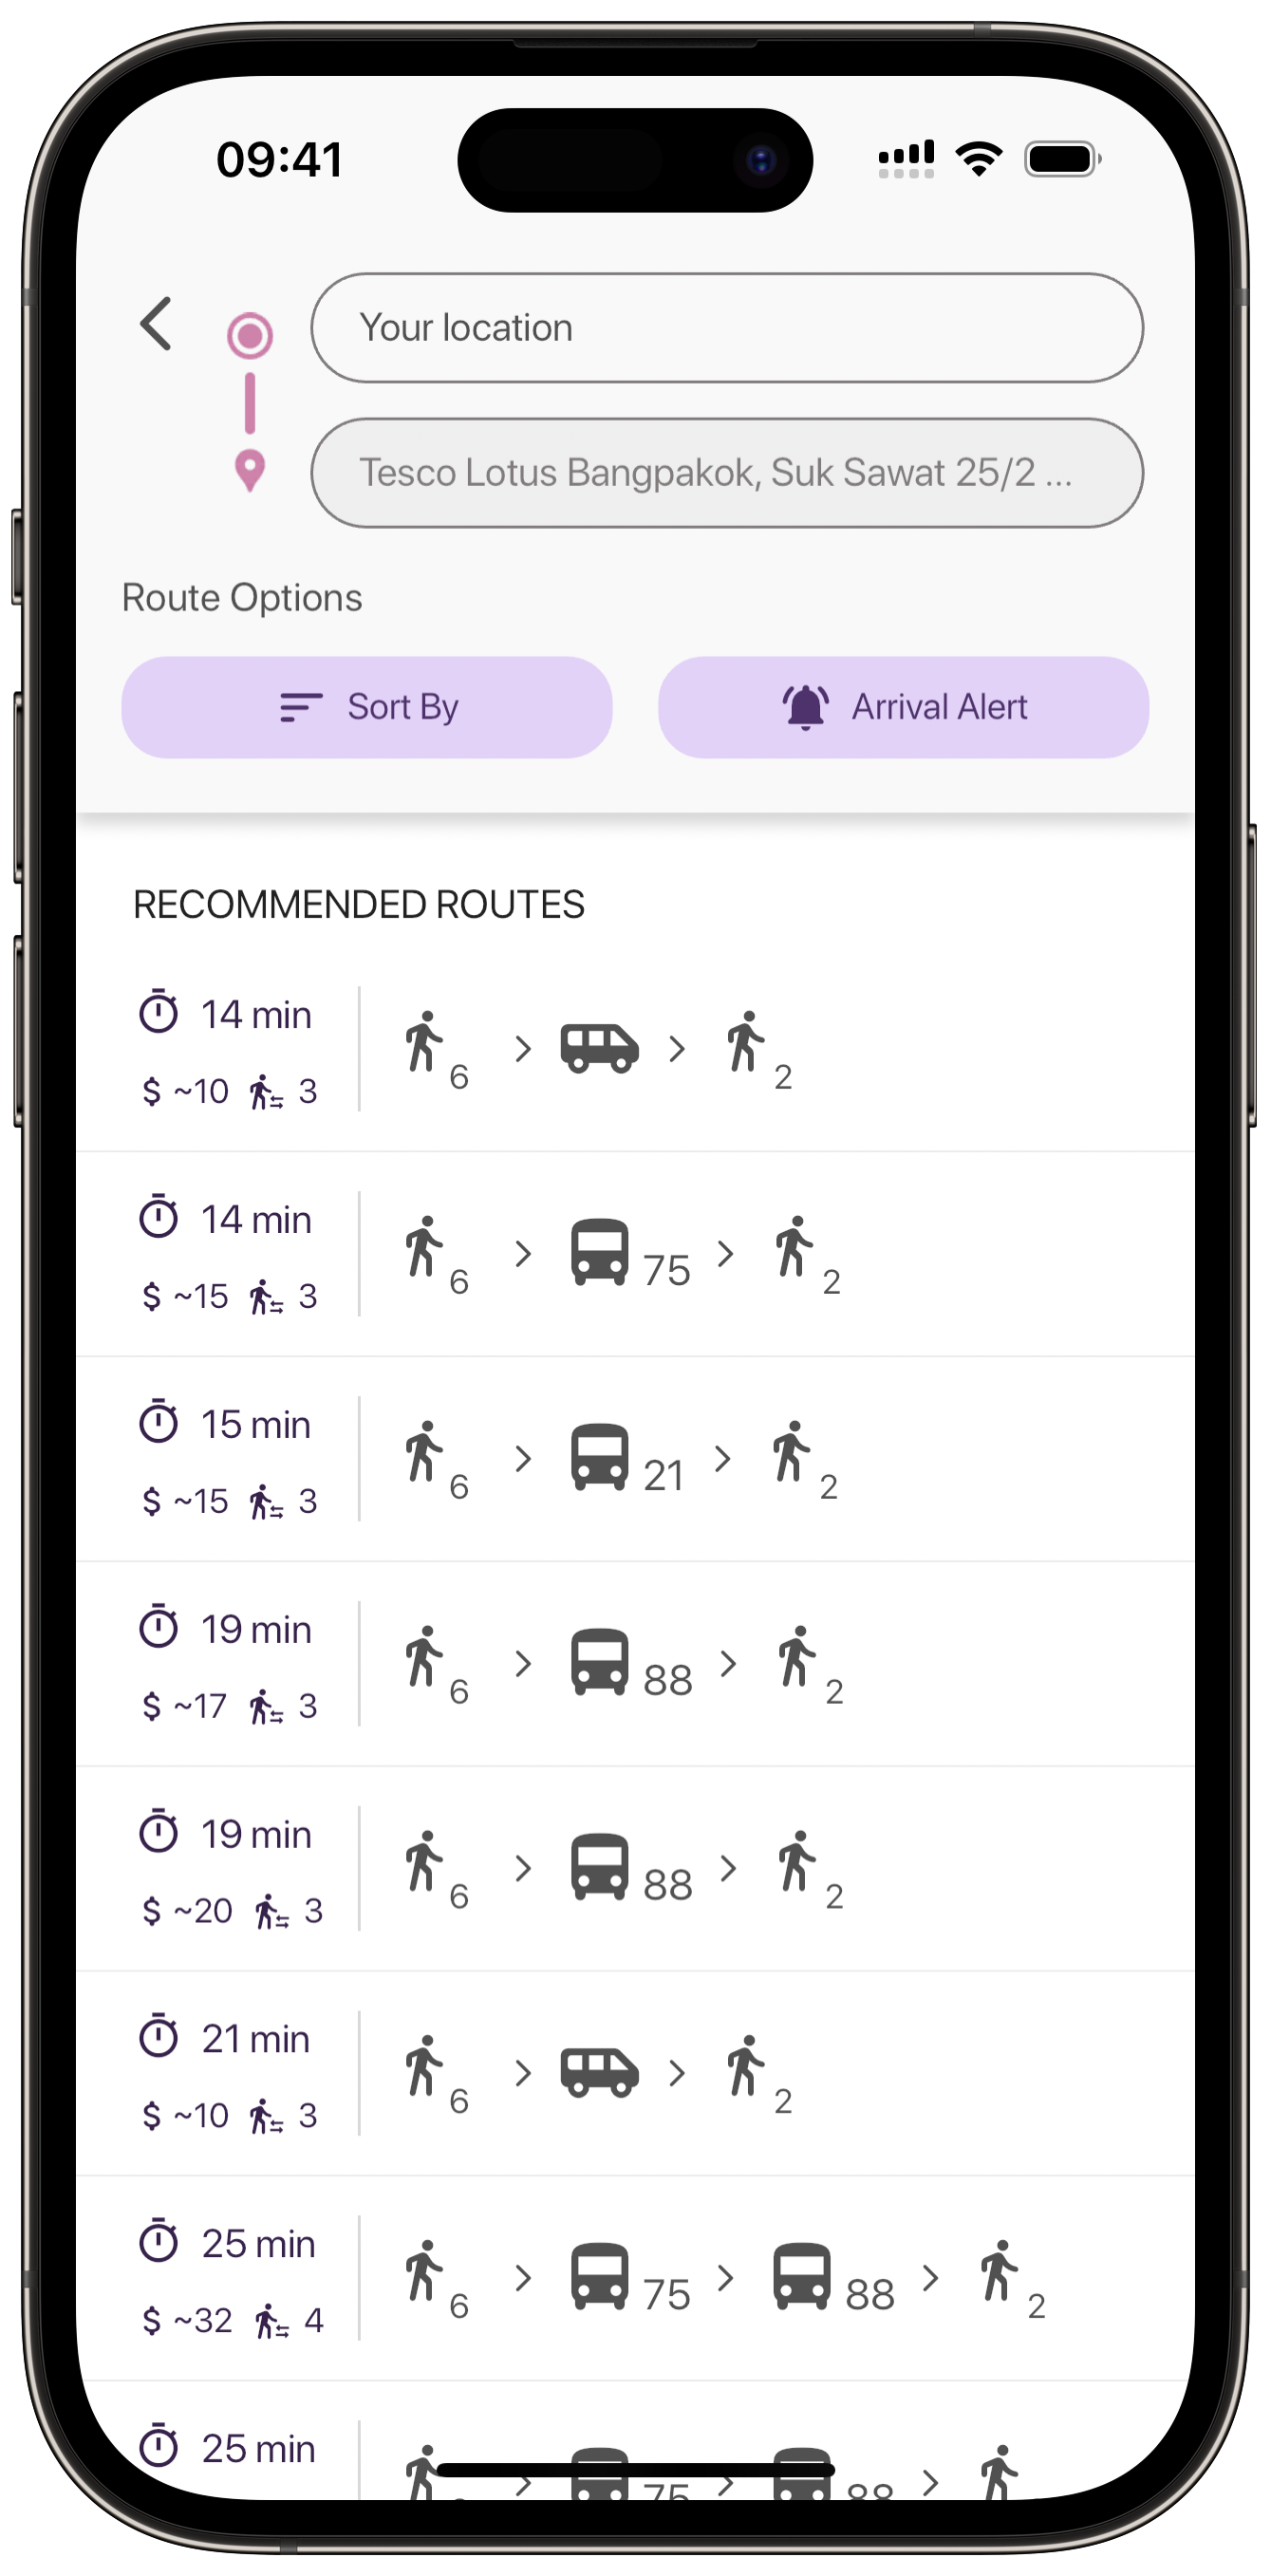
\includegraphics[width=0.5\linewidth]{chapter4/choosing_route_screen.png}
	\caption{Choosing route screen}
	\label{fig:Choosing route screen}
\end{figure}
This figure shows the search route results from the starting location to the destination. All routes are sorted by estimated time of arrival by default and users can see multiple routes to go to the destination.

\newpage
\begin{figure}[!h]
	\centering
	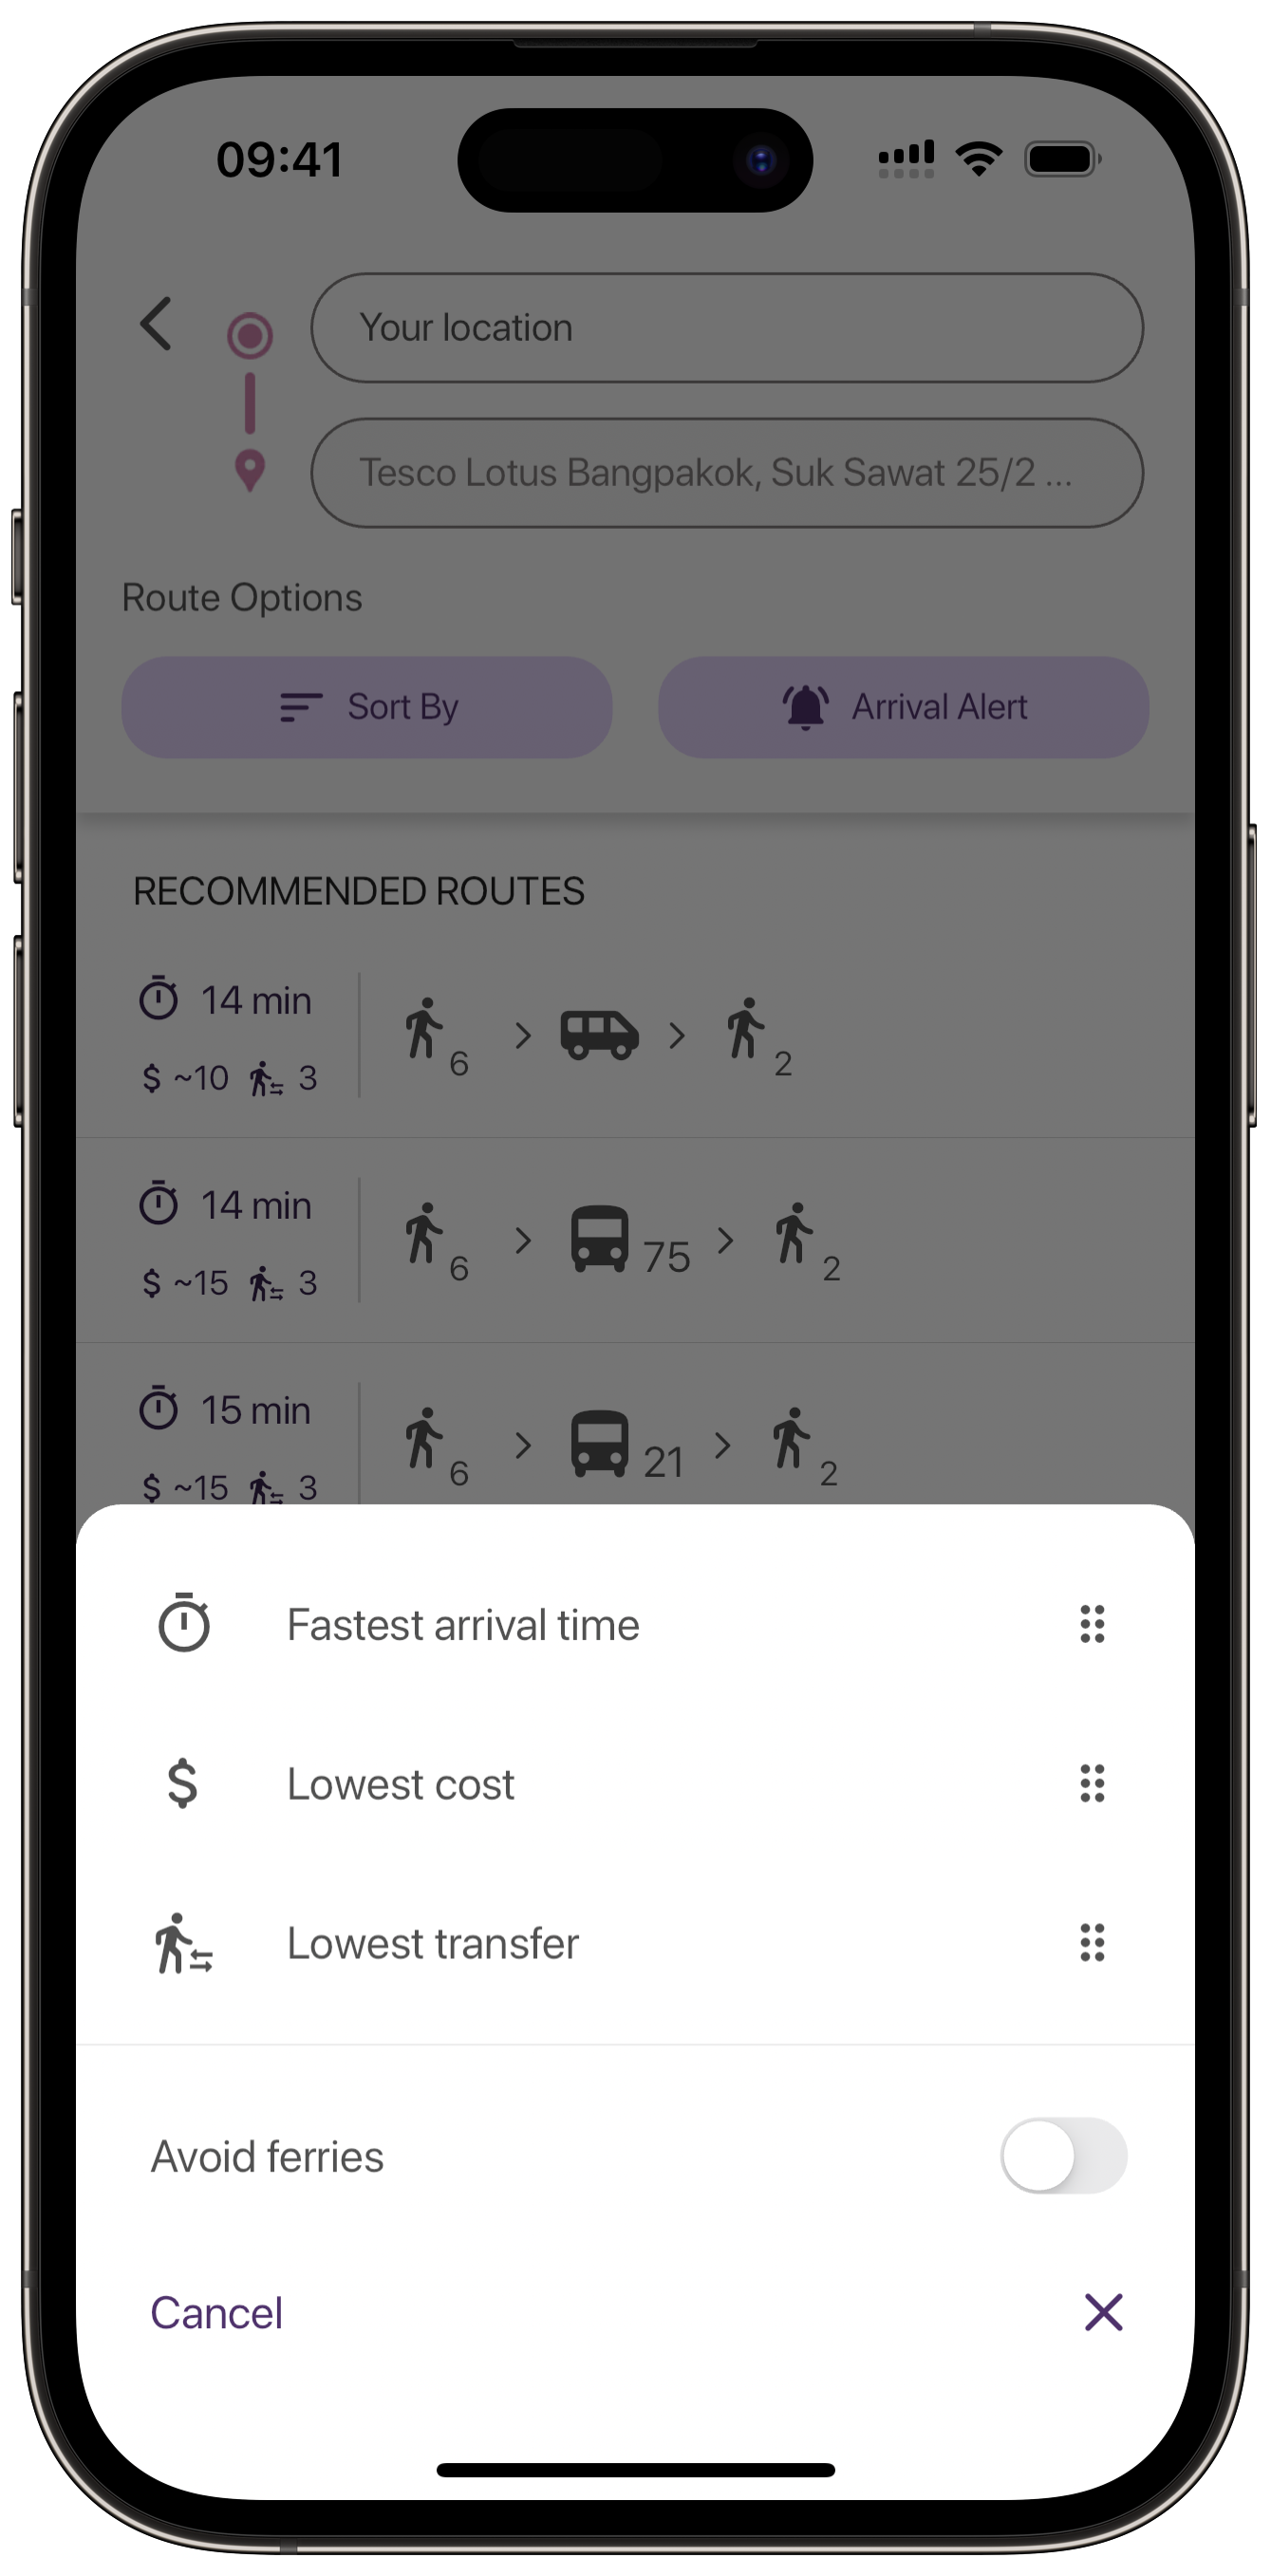
\includegraphics[width=0.5\linewidth]{chapter4/route_options_screen.png}
	\caption{Route options}
	\label{fig:Route options}
\end{figure}
The recommended routes can be sorted according to the user's preferences, such as the fastest arrival time, the cheapest price, the shortest transfer, and the avoid ferry option. 

\newpage
\begin{figure}[!h]
	\centering
	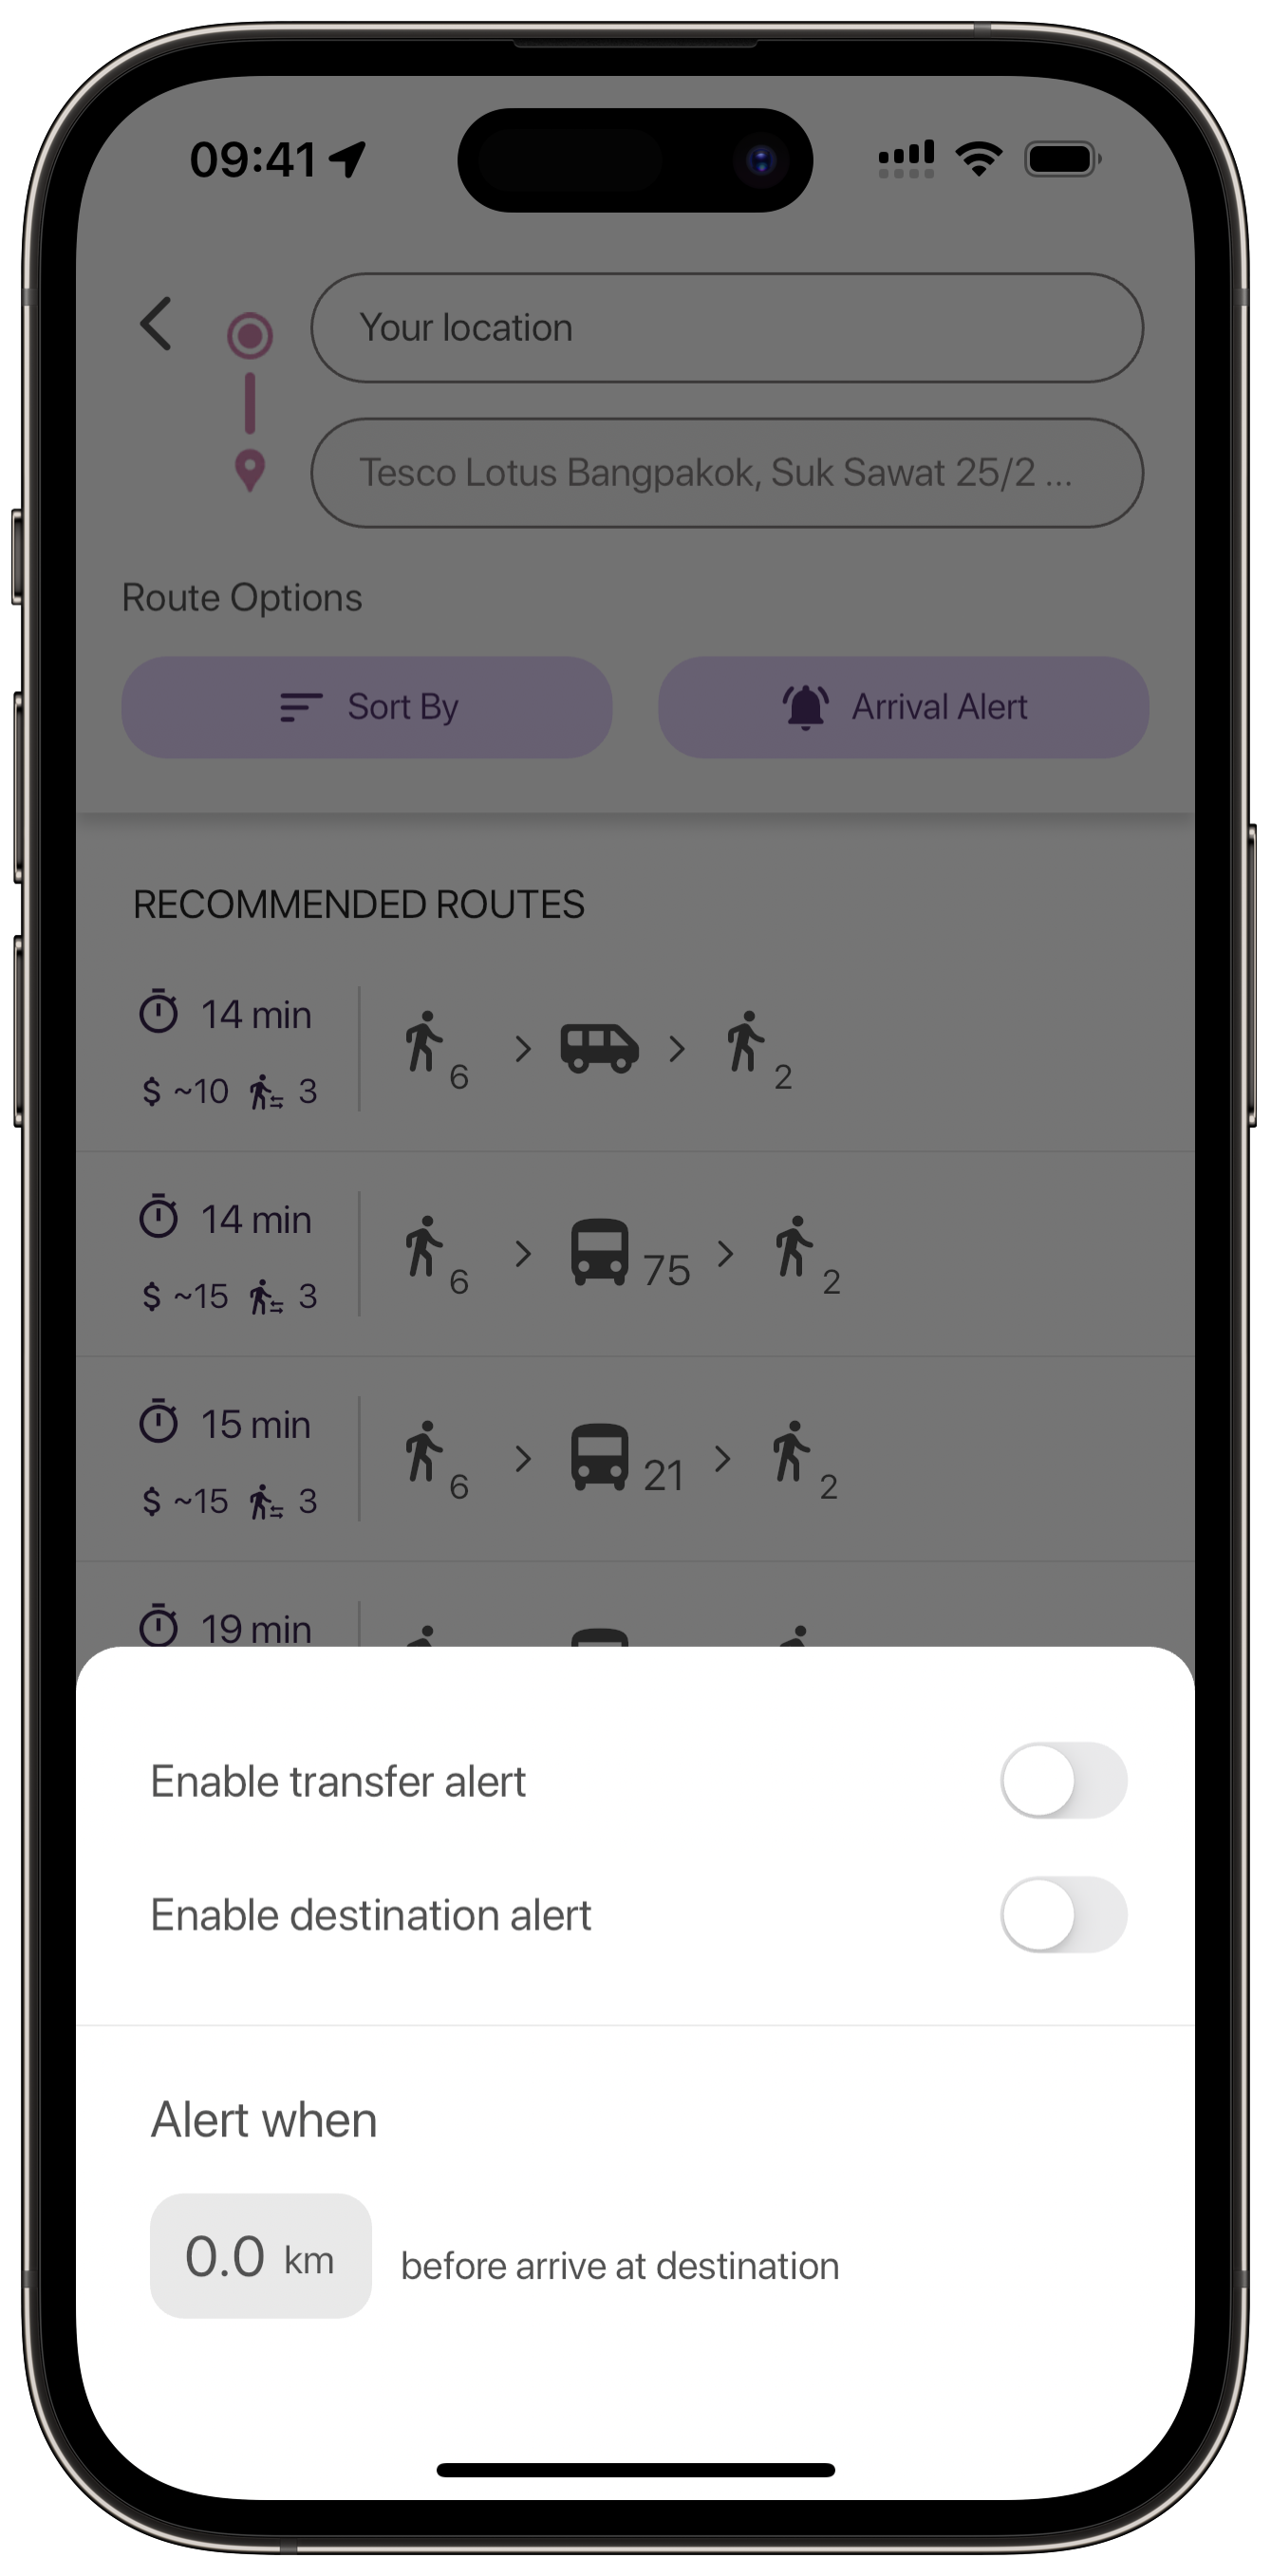
\includegraphics[width=0.5\linewidth]{chapter4/arrival_alert_screen.png}
	\caption{Arrival alert options}
	\label{fig:Arrival alert options}
\end{figure}
There are alerts that can be set when users are nearing the transfer point or the destination which help them reach their destination accurately.

\newpage
\begin{figure}[!h]
	\centering
	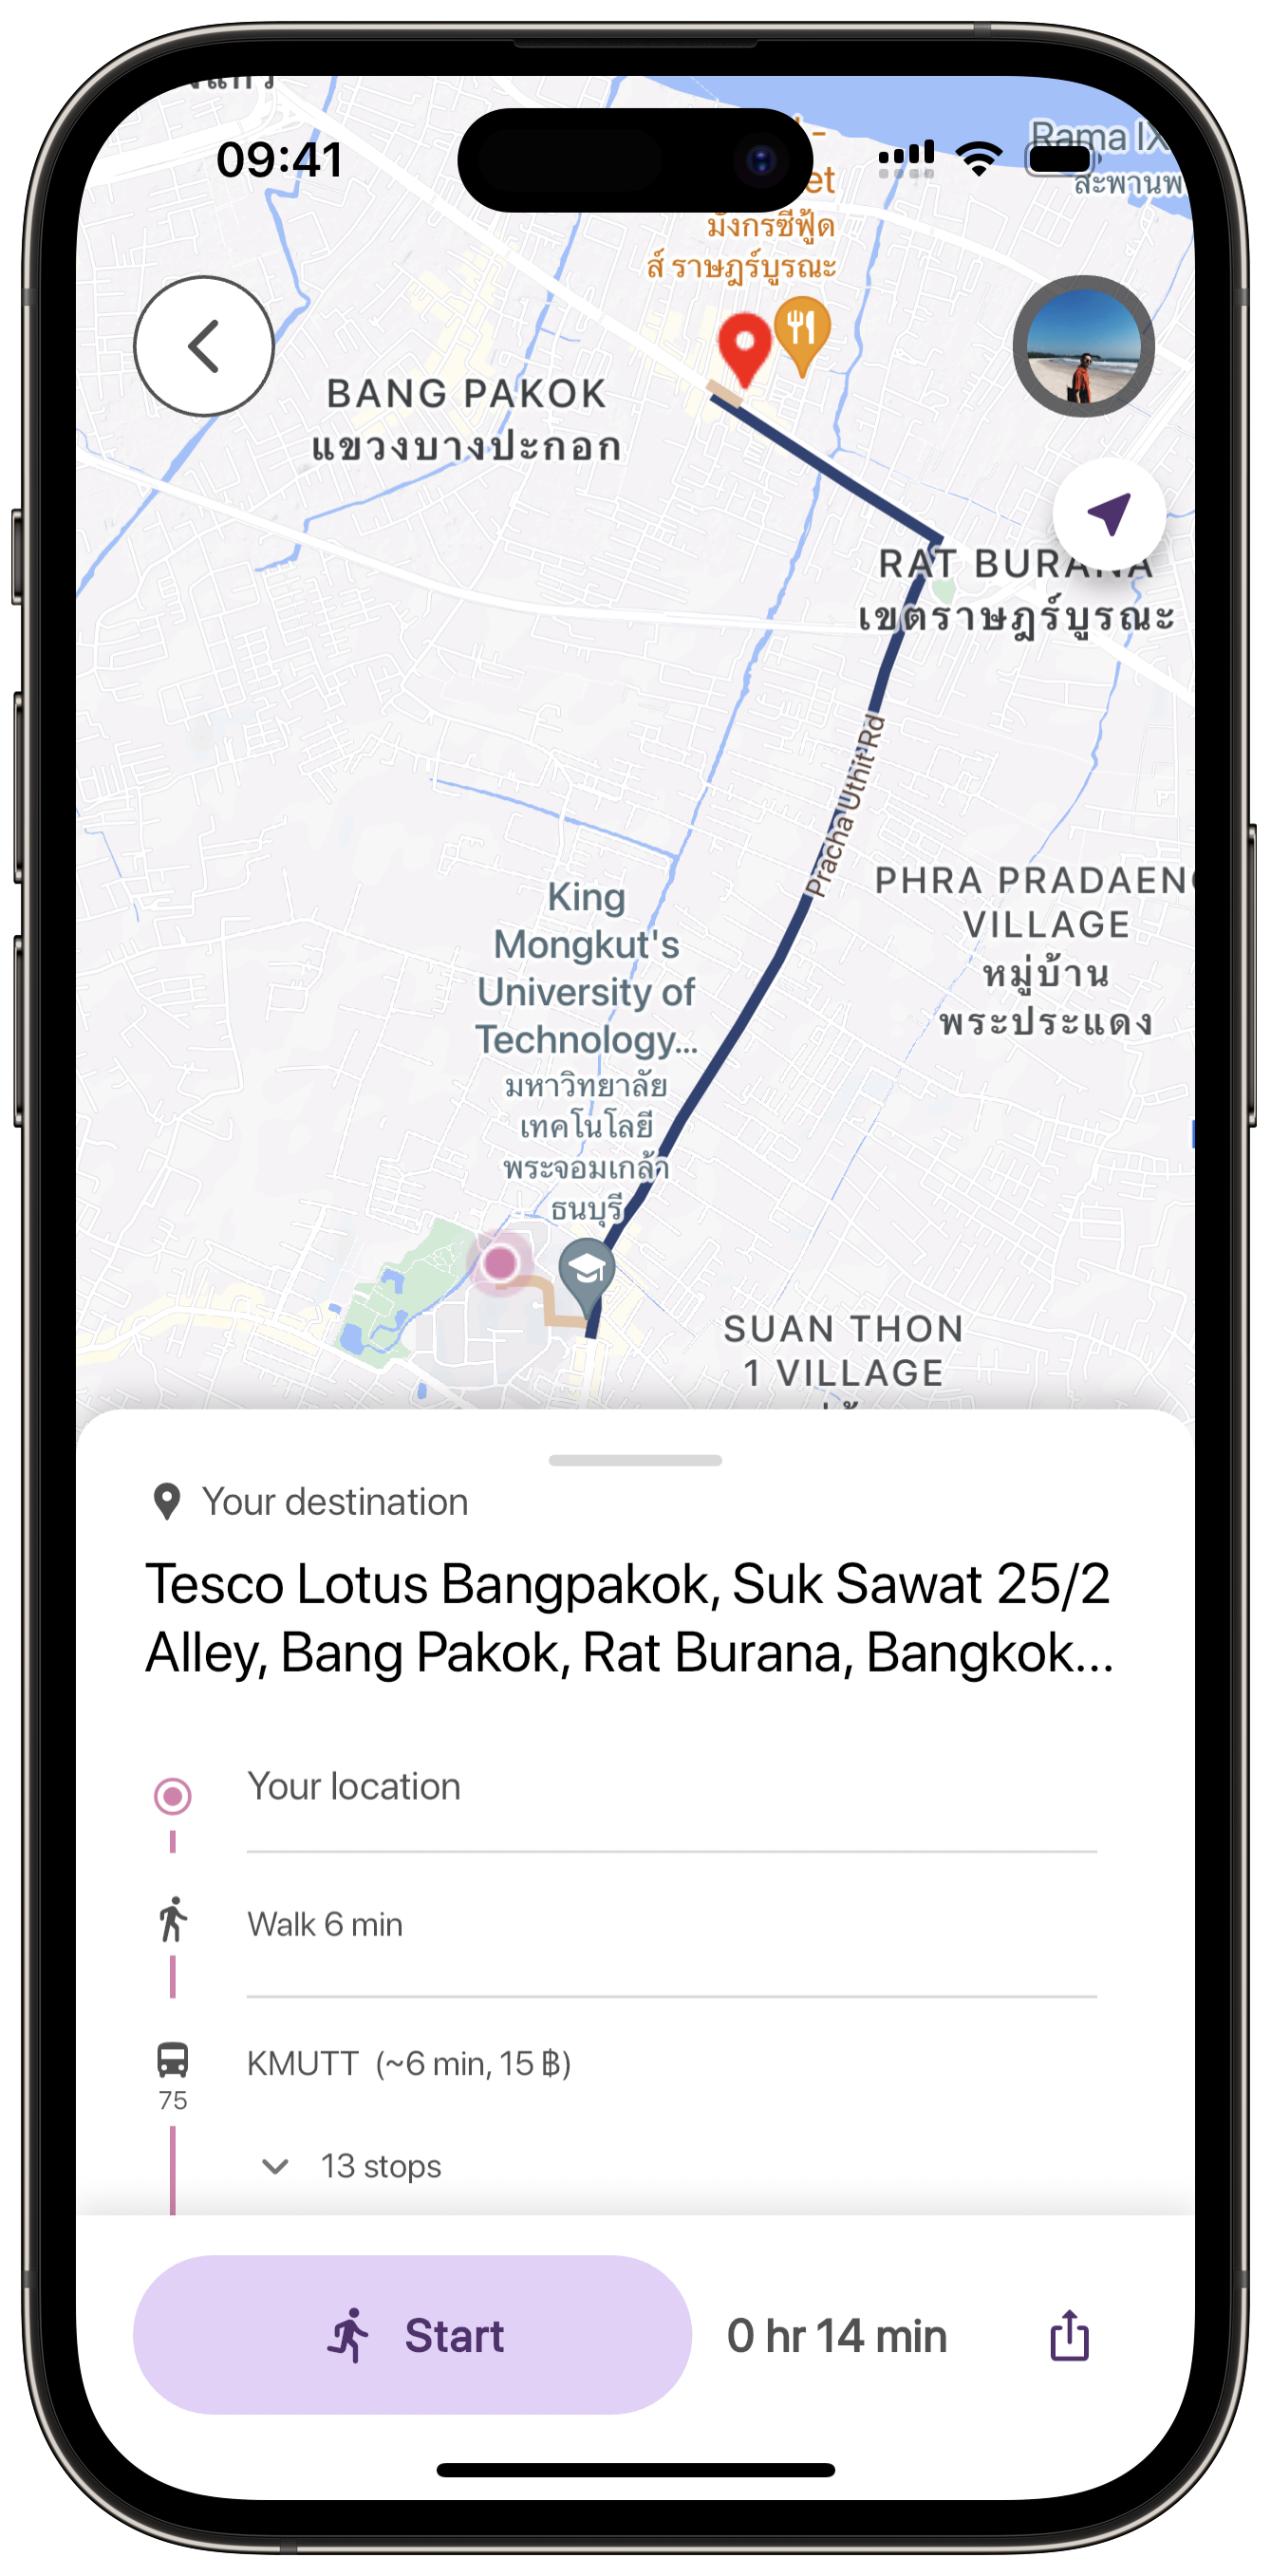
\includegraphics[width=0.5\linewidth]{chapter4/selected_route_screen.png}
	\caption{Selected route screen}
	\label{fig:Selected route screen}
\end{figure}
Users will see the details of the selected route on the map once they select a route from the search route results. From the starting point to the destination, the route polyline is color-coded separately.

\newpage
\begin{figure}[!h]
	\centering
	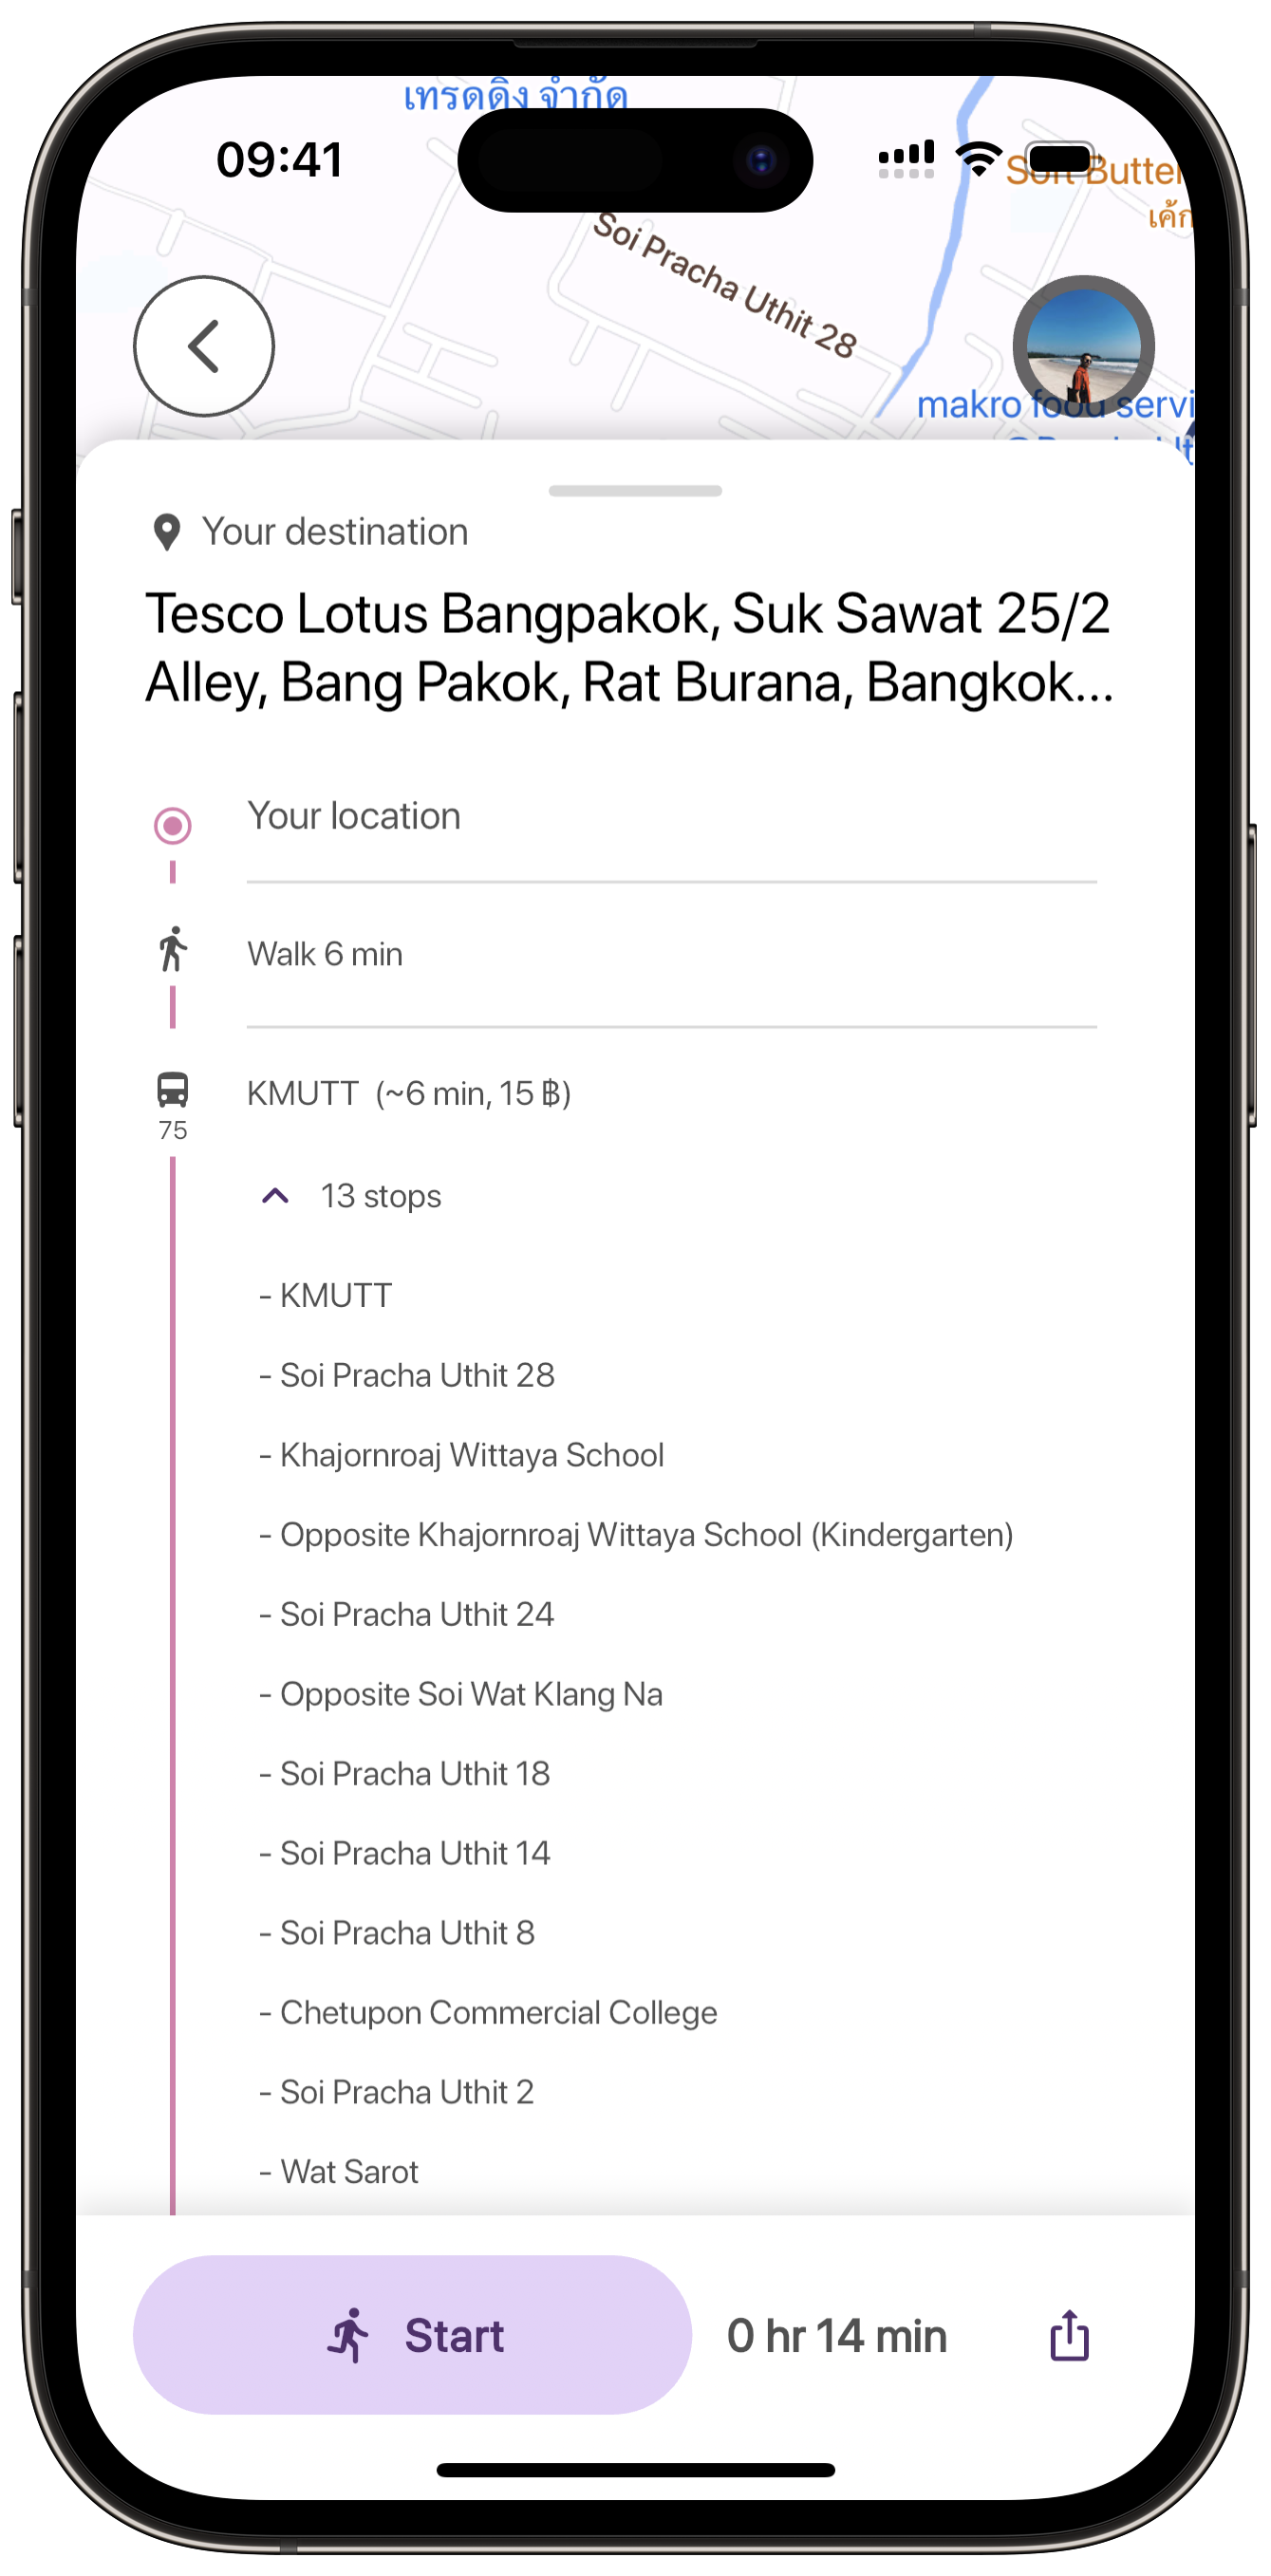
\includegraphics[width=0.5\linewidth]{chapter4/selected_route_detail_screen.png}
	\caption{Selected route detail screen}
	\label{fig:Selected route detail screen}
\end{figure}
After swiping up the bottom sheet, users will see the details of the selected route including cost, estimated time of arrival, and passed stop of each transport type. Users can tap the Start button for starting to real-time navigation or the Share icon to share the selected route with others.

\newpage
\begin{figure}[!h]
	\centering
	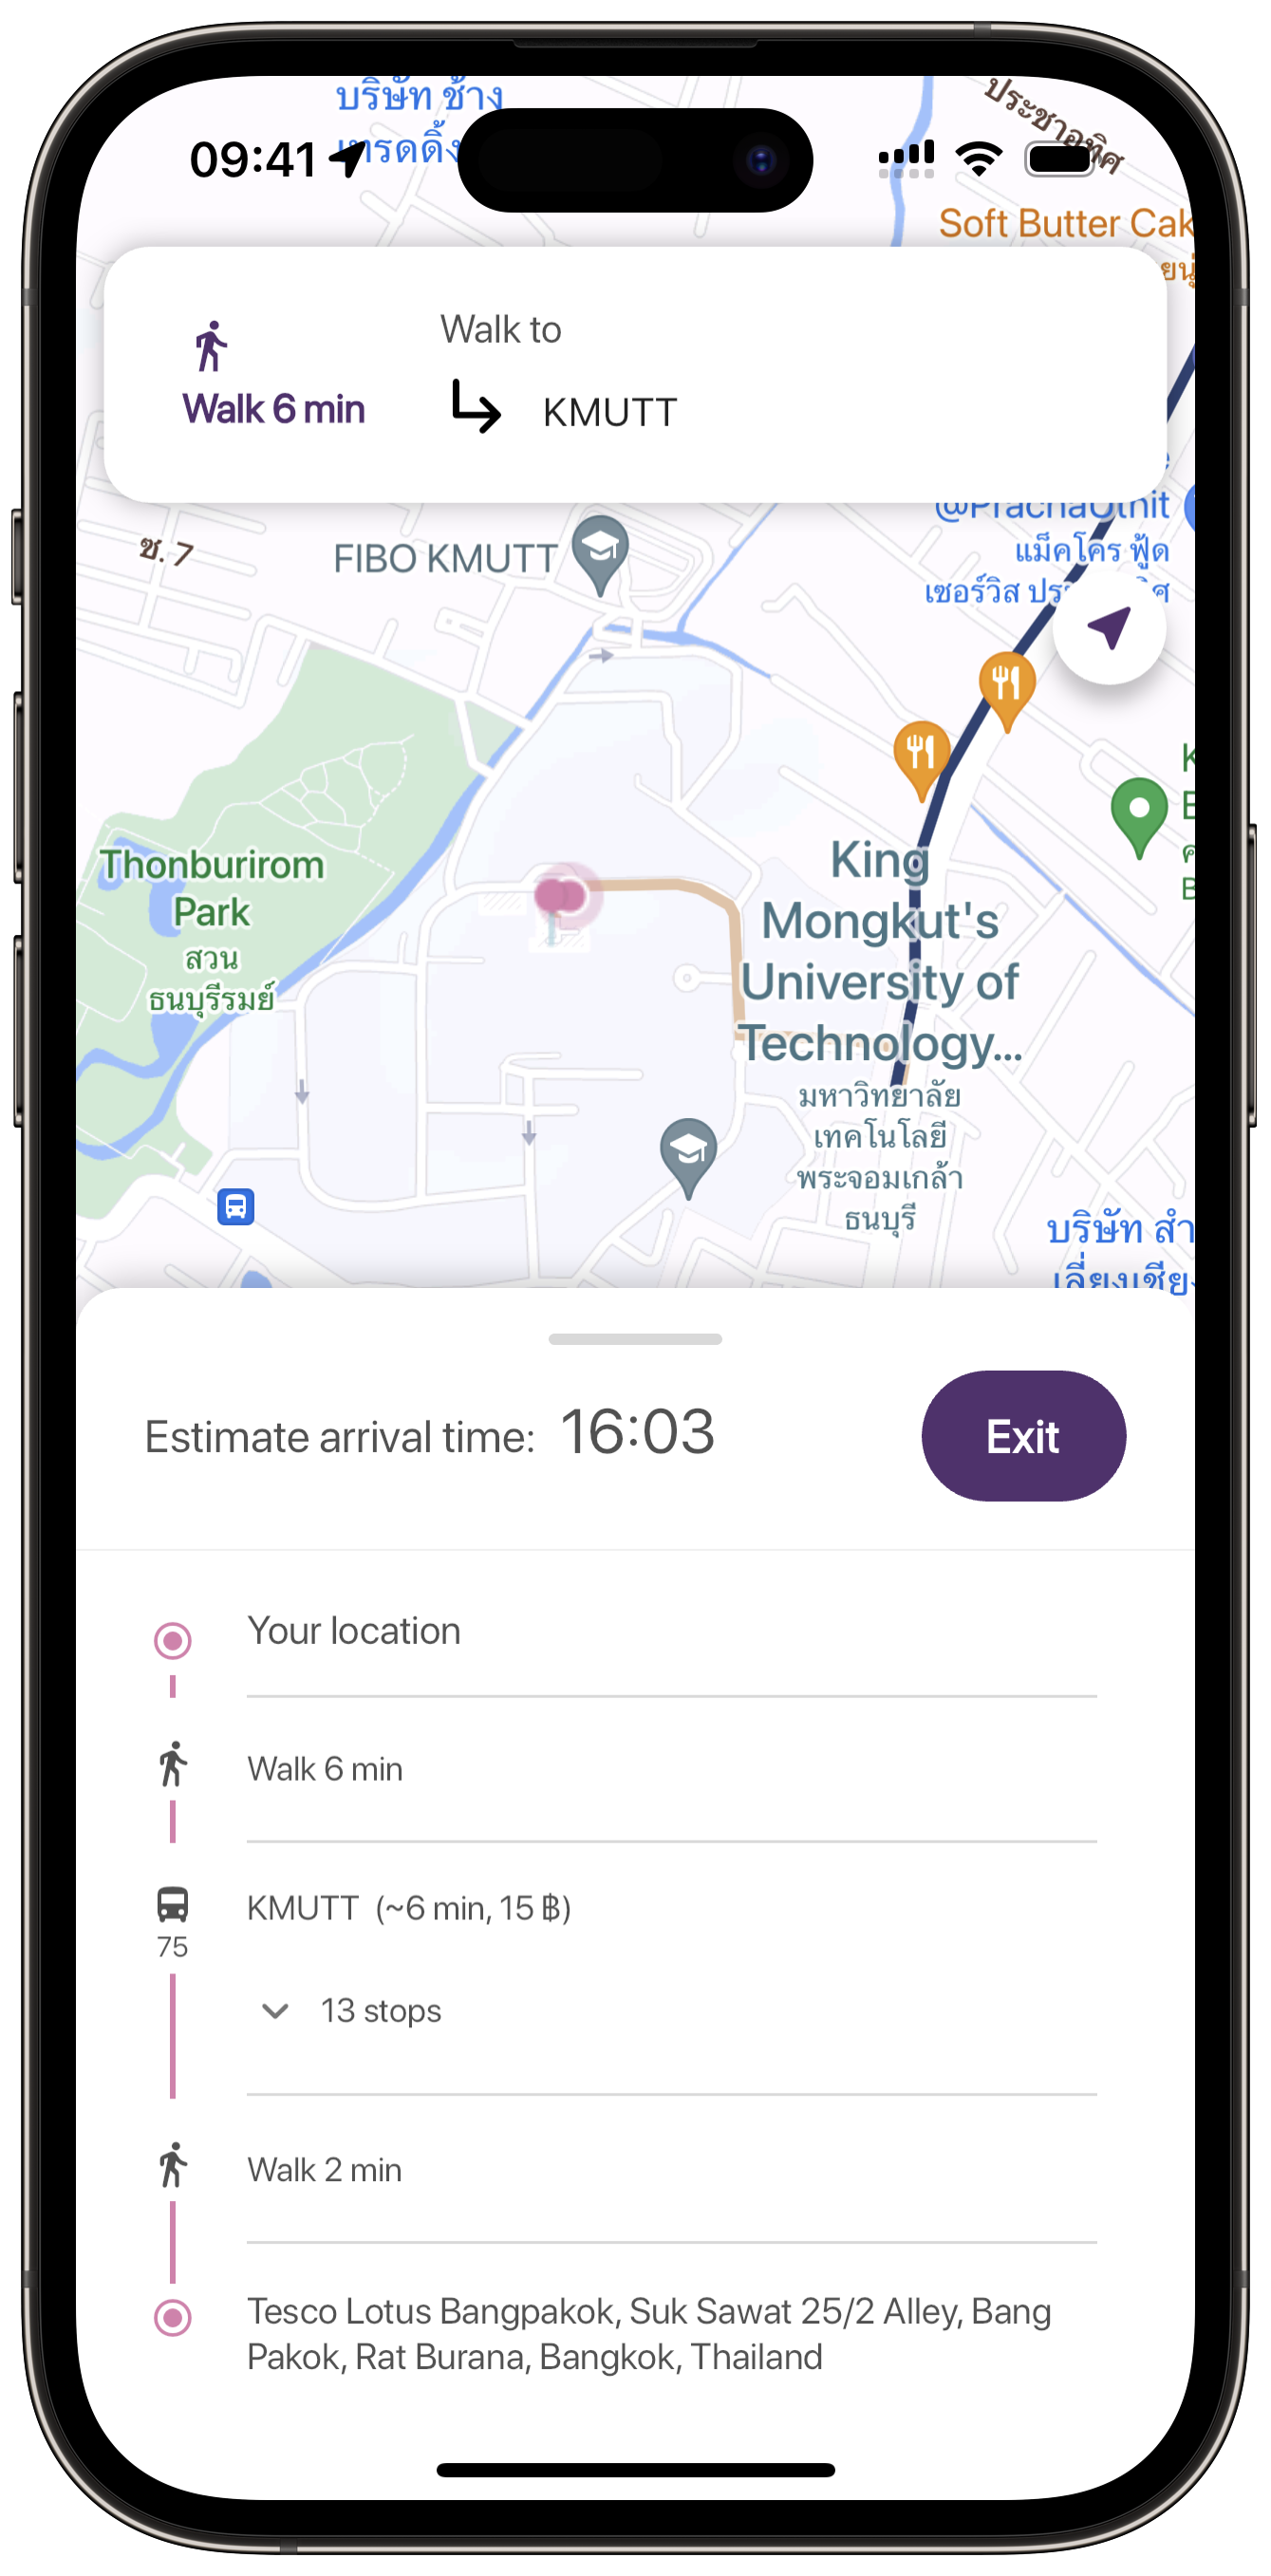
\includegraphics[width=0.5\linewidth]{chapter4/real_time_navigation_screen.png}
	\caption{Real-time navigation screen}
	\label{fig:Real-time navigation screen}
\end{figure}
This screen shows the details of the route in real-time including the current location, estimated arrival time, and the navigation overlay showing the current step with time and the next step at the top of the screen.

\newpage
\begin{figure}[!h]
	\centering
	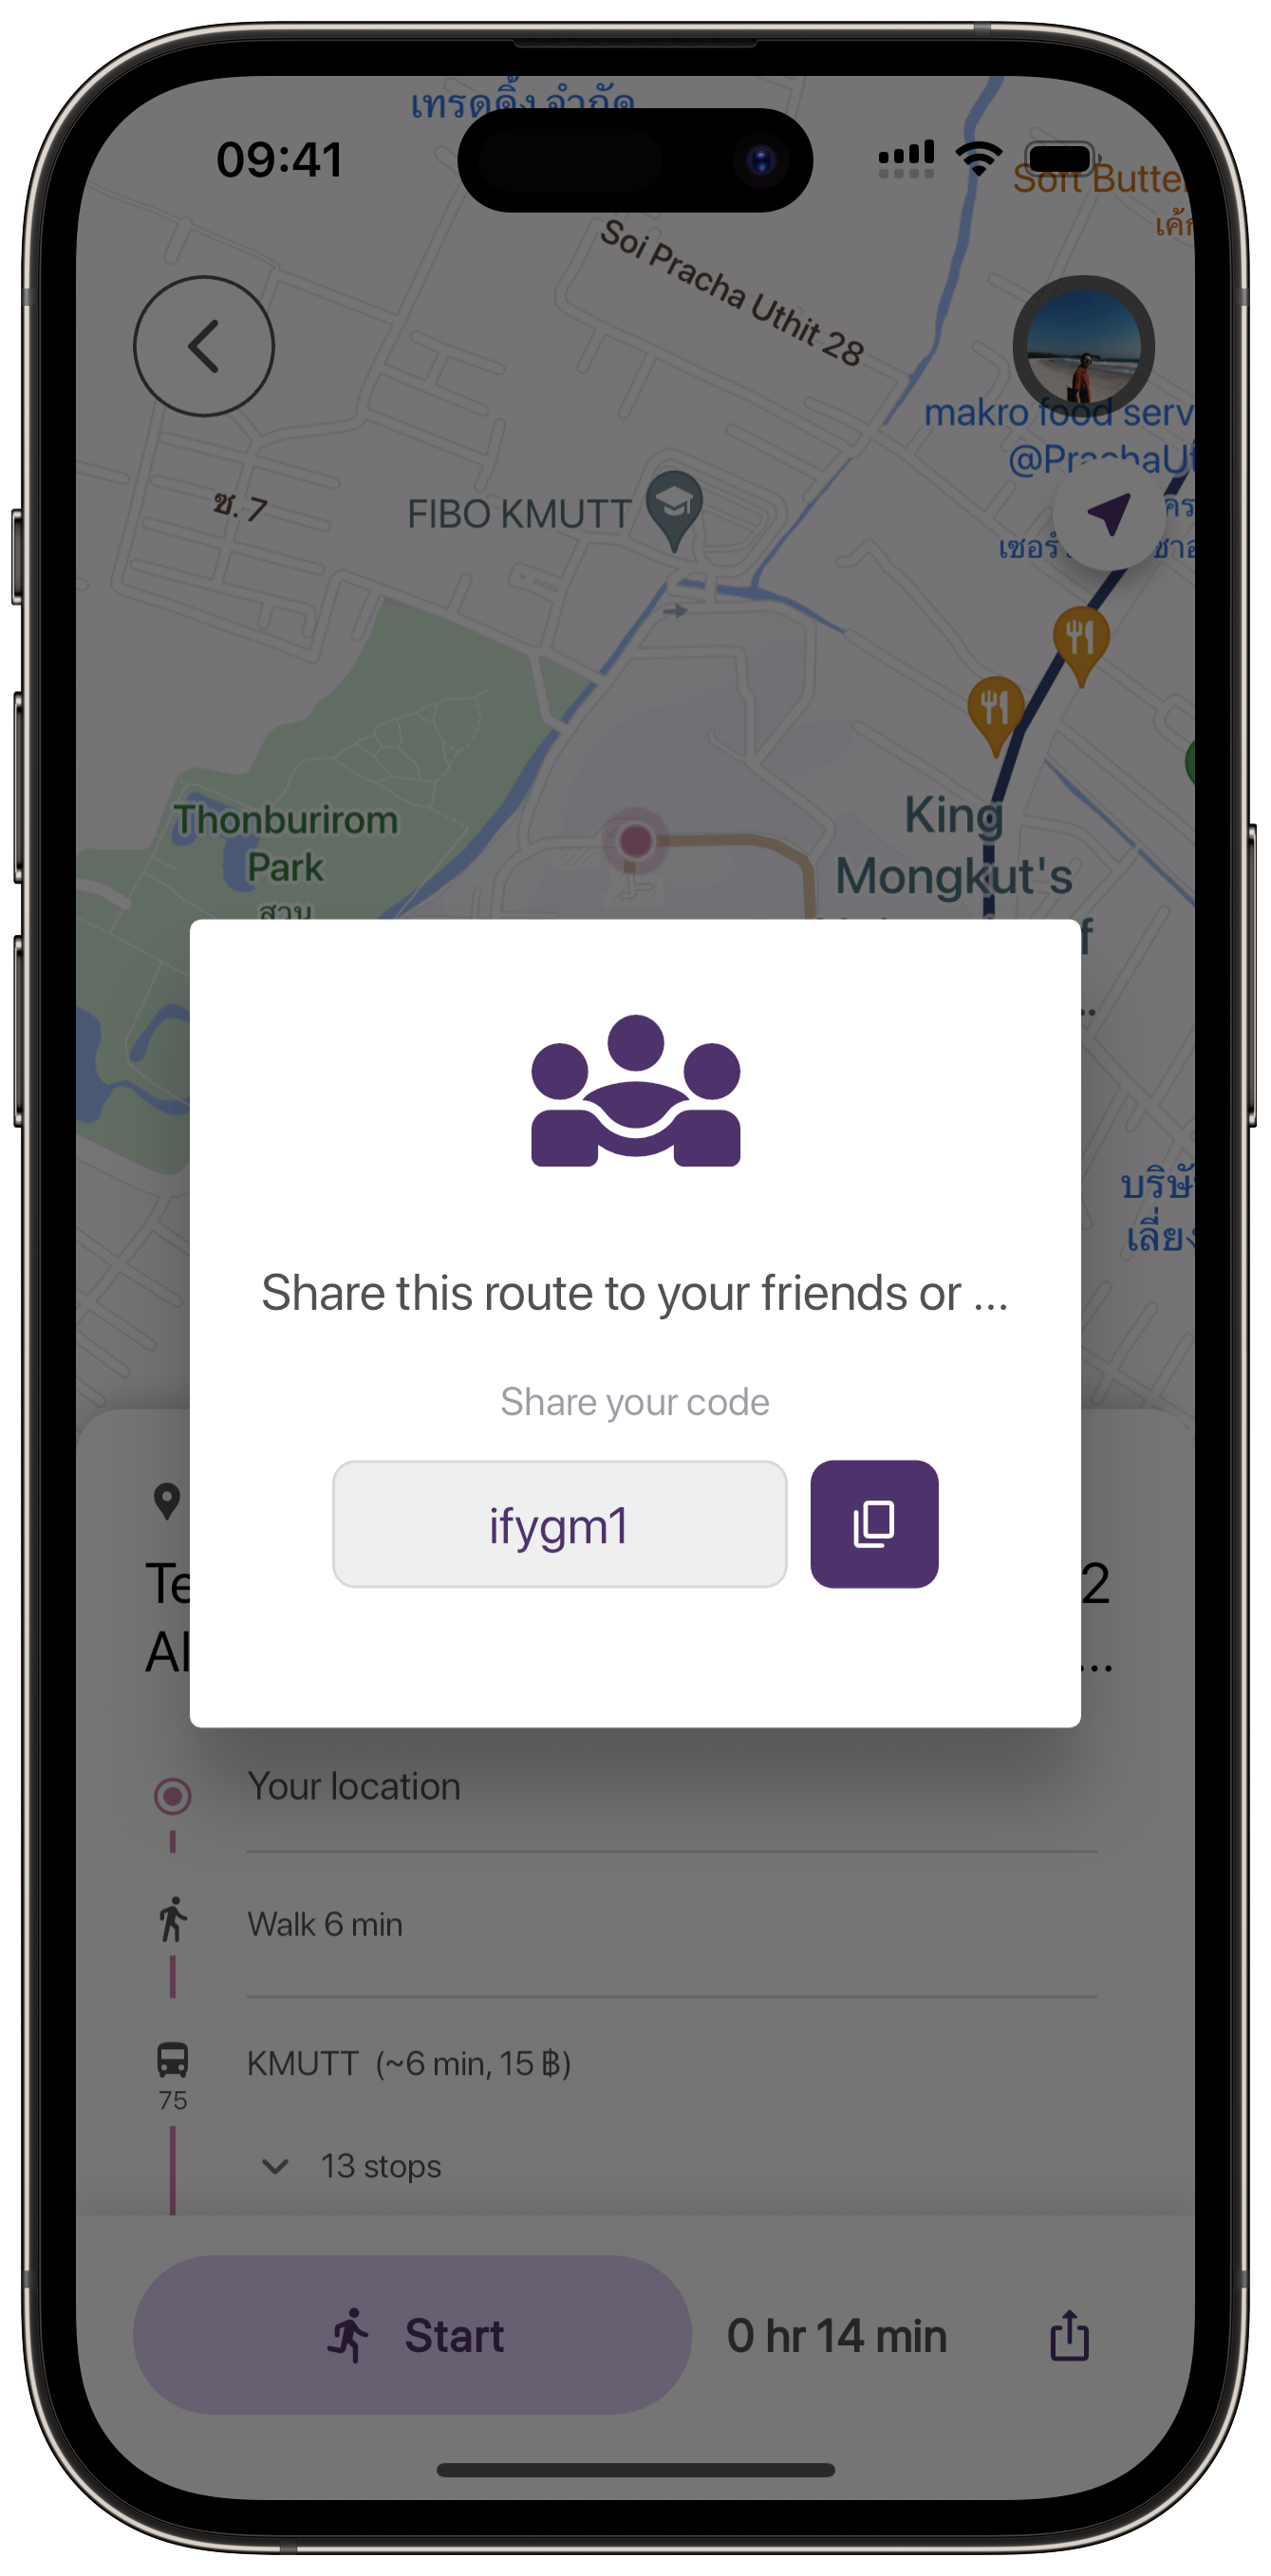
\includegraphics[width=0.5\linewidth]{chapter4/share_route_screen.png}
	\caption{Share route screen}
	\label{fig:Share route screen}
\end{figure}
When users tap the Share button, they will receive the generated code and be able to share the code with others without having to search for the route again. 

\newpage
\begin{figure}[!h]
	\centering
	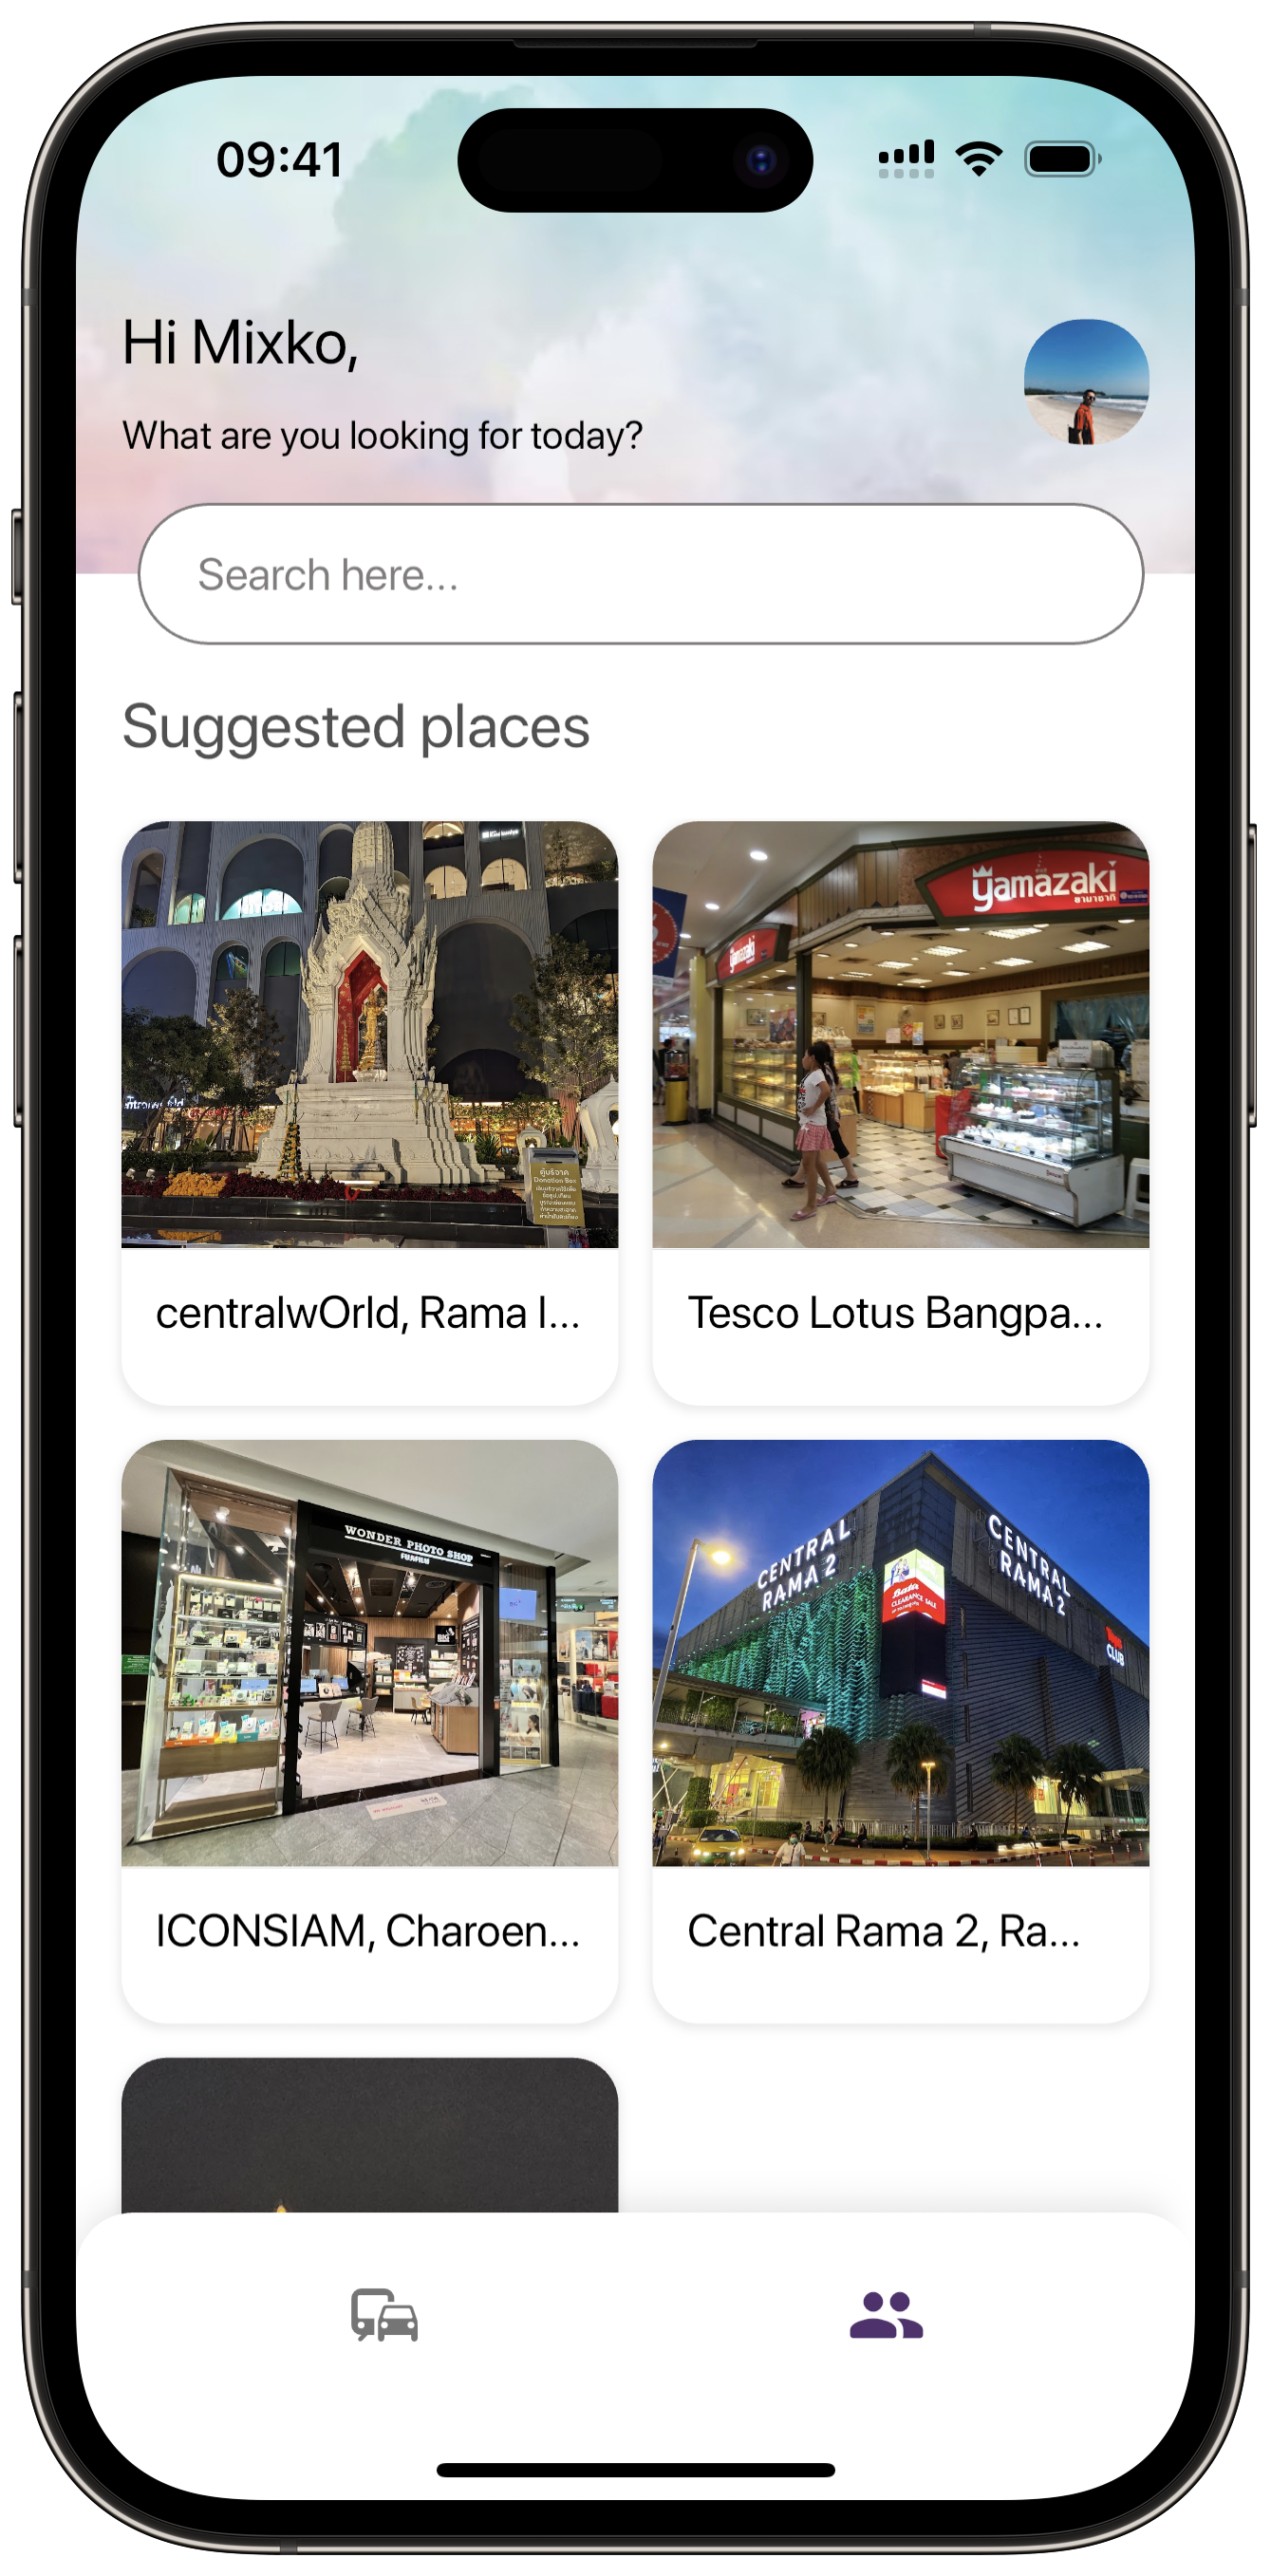
\includegraphics[width=0.5\linewidth]{chapter4/community_screen.png}
	\caption{Community screen}
	\label{fig:Community screen}
\end{figure}
This figure shows the suggested places, which are sorted by how often they are searched, and users can search routes based on the code that is generated by others that will navigate them to the shared routes.

\newpage
\section{Test plan and test result}
\begin{table}[!h]
	\centering
	\resizebox{\linewidth}{!}{%
		\begin{tblr}{
				width = \linewidth,
				colspec = {Q[180]Q[350]Q[492]Q[100]},
				cell{3}{1} = {r=4}{},
				cell{7}{1} = {r=7}{},
				cell{14}{1} = {r=3}{},
				vlines,
				hline{1-3,7,14,17} = {-}{},
				hline{4-6,8-13,15-16} = {2-4}{},
			}
			Module         & Test expectation                                                   & Expected result                                                                                                  & Result  \\
			Authentication & Login with Google                                                  & Successful login to the system with user information provided                                                     & Success \\
			Home page      & Able to navigate between home page and community page              & Can change tab between two page                                                                                  & Success \\
			& Able to see the map with the current user location                  & See the map and correct current location                                                                         & Success \\
			& Able to logout from profile                                        & User is logged out                                                                                               & Success \\
			& Able to navigate to search page/ choose destination                & Navigate to search page correctly                                                                                & Success \\
			Routing        & Able to search for places                                          & User sees the list of places from Google API                                                                      & Success \\
			& Able to sort the route options                                     & User can change the sort by choices to change the travel preferences based on time, cost, and number of transfer & Success \\
			& Able to see the suggested routes when entering start and end location & User sees the list of suggested routes correctly with the details                                                 & Success \\
			& Able to navigate to see each route detail                          & User sees the route detail on the map and modal with travel time and cost                                         & Success \\
			& Able to share the route                                            & User gets a 6-digit code for sharing the route with other users                                                        & Success \\
			& Able to start the trip                                             & User navigates to the routing screen with a map and directions provided                                               & Success \\
			& Able to receive notification when an event happens                     & The system alerts the correct notification                                                                            & Success \\
			Community      & Able to get the exact route when searching by code                    & User navigates to the route detail page correctly                                                                     & Success \\
			& Able to see the suggested places                                   & List of suggested places displays correctly when entering the community page                                             & Success \\
			& Able to navigate to suggested routes page from suggested places    & User navigates to the routes selection page correctly                                                                 & Success 
		\end{tblr}
	}
	\caption{Test plan and result}
	\label{Test plan and result}
\end{table}

\chapter{Summary and suggestions}
\section{Introduction}
This chapter provides a summary of the project, which comprises three parts: project summary, problems encountered and solutions, and suggestions for further development. The first section summarizes and provides the overall results of the project. The second section outlines the problems encountered and proposes solutions to the limitations of the project. Finally, suggestions are provided for the future improvement of the project.

\section{Project summary}
TravelKit is a mobile application that assists individuals in navigating through public transportation options like buses, sky trains, subways, boats, and mini trucks to reach their desired destinations. Users can access information such as pricing, travel duration, and the number of transfers involved in their chosen route. Additionally, the application includes a feature enabling users to share their routes with one another. From the project’s objective and scope, we can create a software that can calculate travel routes, distances, and estimate travel costs with optimizing the suggested routes based on user personal choices.

\section{Problems encountered and solutions}
There are two main problems that we encountered during the project. First problem that we find difficult to cope with is the process of developing mobile application that uses Dart with Flutter as a programming language and framework that we are not quite familiar with. So, we need to learn some new programming styles for the development. The second challenge involves incorporating Neo4j as a graph database, a tool with which we lack prior implementation experience. Consequently, we must familiarize ourselves with the database's query language in order to effectively build our system.

\newpage
\section{Suggestions for further development}
\subsection{Integration of AI in our system}
Currently, our application has a feature that suggest routes based on the users preferences but we can use artificial intelligence to enhance this feature by collecting data from user. We can use that data to predict what sorting preferences user is likely to choose. Furthermore, we can suggest more accurate recommended places to user if we have a proper ai model.
\subsection{Responsive design and implementation}
Currently, our application is working correctly with only certain devices. To support wide variety of mobile and desktop screens, it need revisions in design and implementation to support  the responsive design.
\subsection{High coupling of the data}
Currently, our service has accurate data that we can return route data correctly, but to modify route data, we need to update both in the MongoDB and Neo4j separately which is consequence of manually inserting data to all databases and all relation in Neo4j needs to changed for the updated route.


\bibliographystyle{plain}
\bibliography{references/references}
\cleardoublepage
\addcontentsline{toc}{chapter}{REFERRENCES}

\end{document}